\documentclass[12pt,a4paper]{report}
\usepackage[utf8]{inputenc}
\usepackage{amsfonts}
\usepackage{amsmath}
\usepackage{setspace}
\usepackage{graphicx}
\graphicspath{{../}{./}{../pic/}{../pics/}{pic/}{pics/}{docs/pic/}{docs/pics/}}
\usepackage{array}
\usepackage{fancyhdr}
\usepackage{geometry}
\usepackage{titlesec}
\usepackage{ragged2e}
\usepackage{color}
\usepackage{tabularx}
\usepackage{booktabs}
\usepackage{hyperref}
\usepackage{listings}

\geometry{
a4paper,
total={210mm,297mm},
left=1.15in,
right=0.85in,
top=1.0in,
bottom=1.0in,
}

\makeatletter
\def\@makechapterhead#1{%
  \vspace*{0pt}%
  {\parindent\z@
    \raggedright
    \normalfont
    \Huge\bfseries #1\par\nobreak
    \vskip 20pt}}
\def\@makeschapterhead#1{%
  \vspace*{0pt}%
  {\parindent\z@
    \raggedright
    \normalfont
    \Huge\bfseries #1\par\nobreak
    \vskip 20pt}}
\makeatother

\hypersetup{
    colorlinks=true,
    linkcolor=black,
    citecolor=blue,
    urlcolor=blue
}

\begin{document}

\pagestyle{empty}

%%%%%%%%%%%%%%%%%%% Front Page  %%%%%%%%%%%%%%%%%%%%%%%
\begin{center}
{\large \textbf{Visvesvaraya Technological University, Belagavi – 590018.}}
\begin{figure}[hbtp]
\centering
% NOTE [PHASE 2 ASSET]: pics/vtu.png pending restoration

\includegraphics[width=1.7cm,height=2.4cm]{pics/vtu.png}
\end{figure}

\textbf{PROJECT PHASE-I REPORT}
\par
\textbf{ON}
\par
\vspace{6pt}
{\Large \textbf{Intelligent Academic-to-Industry Transition Support System Using Machine Learning}}
\par
\vspace{8pt}
\par
\textit{\textbf{Submitted in partial fulfillment for the award of degree of }}
\par
\vspace{8pt}
\large \textbf{BACHELOR OF ENGINEERING }
\par
\textbf{in}
\par
\large \textbf{COMPUTER SCIENCE AND ENGINEERING}
\par
\vspace{8pt}
\textit{\textbf{Submitted by}}

\begin{center}
\begin{tabular}{l@{\hspace{2.5cm}}r}
\textbf{\large Shivaraj} & \textbf{4CB23CS141} \\
\textbf{\large Sridharshan} & \textbf{4CB23CS160} \\
\textbf{\large Suhas N R} & \textbf{4CB23CS161} \\
\textbf{\large Vishwas H Acharya} & \textbf{4CB23CS187} \\
\end{tabular}
\end{center}

\vspace{8pt}
\textit{\textbf{Under the Guidance of}}
\par
\vspace{6pt}
\textbf{Ms. Sushma}
\par
\vspace{2pt}
\normalsize {Assistant Professor, Department of CS\&E}
\par
\begin{figure}[hbtp]
\centering
% NOTE [PHASE 2 ASSET]: pics/CEC-logo.jpg pending restoration

\includegraphics[scale=0.6]{pics/CEC-logo.jpg}\textbf{}
\end{figure}
\large \textbf{DEPARTMENT OF COMPUTER SCIENCE AND ENGINEERING}
\par \Large \textbf{CANARA ENGINEERING COLLEGE}

{\large{(An Autonomous Institution, Under VTU Belagavi, Recognized by AICTE, Accredited by NBA (CSE, ISE, ECE) and NAAC 'A' GRADE)}}
\par
{\large \textbf{Sudhindra Nagar, Benjanapadavu, Mangaluru - 574219, Karnataka.}}
\par 
{\Large \textbf{A.Y 2025-26}}
\end{center}
\newpage

%%%%%%%%%%%%%%%%%%%%%%%%%% Certificate Page %%%%%%%%%%%%%%%

\begin{center}
\LARGE \textbf{CANARA ENGINEERING COLLEGE}
\par

\par \large{(An Autonomous Institution, Under VTU Belagavi, Recognized by AICTE, Accredited by NBA (CSE, ISE, ECE) and NAAC 'A' GRADE)}
\par \vspace{3pt}
\large \textbf{Sudhindra Nagar, Benjanapadavu, Mangaluru - 574219, Karnataka.}
\par \vspace{12pt}  
\par
\large \textbf{DEPARTMENT OF COMPUTER SCIENCE AND ENGINEERING}
\par
\begin{figure}[hbtp]
\centering
% NOTE [PHASE 2 ASSET]: pics/CEC-logo.jpg pending restoration

\includegraphics[scale=0.5]{pics/CEC-logo.jpg}
\end{figure}

{\Large \textbf{CERTIFICATE}}
\end{center}
\justifying
\par
\setstretch{1.2}
\noindent 
Certified that the Project work Phase-I entitled \textbf{``Intelligent Academic-to-Industry Transition Support System Using Machine Learning''} carried out by\vspace{2pt} 
\par
\noindent 
\begin{center}
\begin{tabular}{l@{\hspace{2.5cm}}r}
\textbf{\large Shivaraj} & \textbf{4CB23CS141} \\
\textbf{\large Sridharshan} & \textbf{4CB23CS160} \\
\textbf{\large Suhas N R} & \textbf{4CB23CS161} \\
\textbf{\large Vishwas H Acharya} & \textbf{4CB23CS187} \\
\end{tabular}
\end{center}
\noindent
the bonafide students of VI semester COMPUTER SCIENCE AND ENGINEERING in partial fulfillment for the award of Bachelor of Engineering in COMPUTER SCIENCE AND ENGINEERING of the Visvesvaraya Technological University, Belagavi during the year 2025-2026. It is certified that all corrections/suggestions given during internal reviews are included for Internal Assessment. The Project Phase-I report has been approved as it satisfies the academic requirements in respect of Phase-I Project work prescribed for the said degree. 

\par
\vspace{0.35in}
\setstretch{1.15}

\begin{tabularx}{0.98 \textwidth} { 
   >{\raggedright\arraybackslash}X 
   >{\centering\arraybackslash}X
   >{\raggedleft\arraybackslash}X }
     \textbf{Ms. Sushma} & \textbf{Dr. Vinay P} & \textbf{Dr. Rajgopal K T} \\
     Project Guide & Project-Coordinator & HoD \\
\end{tabularx}

\par
\vspace{0.3in}
\setstretch{1.15}

\begin{tabularx}{0.98 \textwidth} {  
   >{\raggedright\arraybackslash}X 
   >{\raggedleft\arraybackslash}X}
    \textbf{Dr. Demian Antony D'Mello} & \textbf{Principal} \\
    Dean-Academics  & Canara Engineering College \\
\end{tabularx}

\vspace{0.2in}
\begin{center}
\large \textbf{Internal / External Viva}:
\end{center}
\begin{flushleft}
\begin{normalsize}Examiner's Name \end{normalsize}
\hspace{7.5cm}
\begin{normalsize}Signature with Date\end{normalsize}
\end{flushleft}

\begin{flushleft}
1. \ldots\ldots\ldots\ldots\ldots\ldots\ldots\ldots\ldots\ldots\ldots\ldots \hspace{4.2cm} \ldots\ldots\ldots\ldots\ldots\ldots\ldots\ldots\ldots\ldots\ldots\ldots 
\par
\vspace{0.15in}	
2. \ldots\ldots\ldots\ldots\ldots\ldots\ldots\ldots\ldots\ldots\ldots\ldots \hspace{4.2cm} \ldots\ldots\ldots\ldots\ldots\ldots\ldots\ldots\ldots\ldots\ldots\ldots 
\end{flushleft}
\newpage

%%%%%%%%%%%%%%%%%%%%%% Declaration Page %%%%%%%%%%%%%%%%%
\begin{center}
\LARGE \textbf{CANARA ENGINEERING COLLEGE}
\par
\par \large{(An Autonomous Institution, Under VTU Belagavi, Recognized by AICTE, Accredited by NBA (CSE, ISE, ECE) and NAAC 'A' GRADE)}
\par \vspace{3pt}
\large \textbf{Sudhindra Nagar, Benjanapadavu, Mangaluru - 574219, Karnataka.}
\par \vspace{12pt}  
\par
\large \textbf{DEPARTMENT OF COMPUTER SCIENCE AND ENGINEERING}
\par
\begin{figure}[hbtp]
\centering
% NOTE [PHASE 2 ASSET]: pics/CEC-logo.jpg pending restoration

\includegraphics[scale=0.5]{pics/CEC-logo.jpg}
\end{figure}

{\Large \textbf{DECLARATION}}
\end{center}
\justifying
\par

\setstretch{1.5}
\noindent We hereby declare that our entire work embodied in this Project Report titled \textbf{``Intelligent Academic-to-Industry Transition Support System Using Machine Learning''} has been carried out at CANARA ENGINEERING COLLEGE, Mangaluru under the supervision of \textbf{Ms. Sushma}, Assistant Professor, Department of Computer Science and Engineering, for the award of \textbf{Bachelor of Engineering} in \textbf{COMPUTER SCIENCE AND ENGINEERING}. This report has not been submitted to this or any other University for the award of any other degree. \\
\vspace{0.35in}

\begin{tabularx}{0.95 \textwidth} { 
   >{\raggedleft\arraybackslash}X }
    \begin{tabular}{l@{\hspace{1cm}}r}
    \textbf{\large Shivaraj (4CB23CS141)} & \ldots\ldots\ldots\ldots\ldots\ldots\ldots\ldots \\
    \textbf{\large Sridharshan (4CB23CS160)} & \ldots\ldots\ldots\ldots\ldots\ldots\ldots\ldots \\
    \textbf{\large Suhas N R (4CB23CS161)} & \ldots\ldots\ldots\ldots\ldots\ldots\ldots\ldots \\
    \textbf{\large Vishwas H Acharya (4CB23CS187)} & \ldots\ldots\ldots\ldots\ldots\ldots\ldots\ldots \\
    \end{tabular}\\
\end{tabularx}

%%%%%%%%%%%%%%%%%%%%%%%%%% Acknowledgement %%%%%%%%%%%%%%%

\newpage
\setstretch{1.2}
\chapter*{Acknowledgement}
\addcontentsline{toc}{chapter}{\numberline{}Acknowledgement}
We dedicate this page to acknowledge and thank those responsible for the shaping of this project. Without their constant guidance, valuable critique, and encouragement, constructing this project report would not have been so smooth and efficient.
\par
\vspace{0.15in}
\noindent We sincerely thank our Project Guide \textbf{Ms. Sushma}, Assistant Professor, Department of Computer Science and Engineering, for her keen guidance, constructive suggestions, and continuous supervision which helped us navigate technical roadblocks and complete this phase successfully.
\par
\vspace{0.15in}
\noindent We also convey our sincere gratitude to our Project Coordinator \textbf{Dr. Vinay P}, Department of Computer Science and Engineering, for his consistent encouragement, milestone scheduling, and insightful reviews during internal assessments.
\par
\vspace{0.15in}
\noindent We owe a profound gratitude to \textbf{Dr. Rajgopal K T}, Head of the Department, Computer Science and Engineering, whose constant encouragement, administrative support, and academic guidance enabled us to work in an inspiring environment.
\par
\vspace{0.15in}
\noindent We also take this opportunity to thank our Dean Academics \textbf{Dr. Demian Antony D'Mello} and our respected Principal for providing state-of-the-art infrastructural facilities and computational resources to carry out our project work.
\par
\vspace{0.15in}
\noindent We express our gratitude to all teaching and non-teaching staff of the Department of Computer Science and Engineering for their direct and indirect support throughout the course of this work. Finally, we convey our deepest appreciation to our parents and friends for their enduring patience, moral support, and enthusiasm.
\par
\vspace{0.3in}
\begin{tabularx}{0.95 \textwidth} { 
   >{\raggedleft\arraybackslash}X }
    \begin{tabular}{l}
    \textbf{Shivaraj (4CB23CS141)} \\
    \textbf{Sridharshan (4CB23CS160)} \\
    \textbf{Suhas N R (4CB23CS161)} \\
    \textbf{Vishwas H Acharya (4CB23CS187)} \\
    \end{tabular}\\
\end{tabularx}

%%%%%%%%%%%%%%%%%%%%%%%%%% Abstract %%%%%%%%%%%%%%%%%%%%%%%%%%%%%

\pagestyle{plain}
\setstretch{1.5}
\pagenumbering{roman}
\chapter*{Abstract}
\addcontentsline{toc}{chapter}{\numberline{}Abstract}
Graduating engineering students frequently encounter severe hurdles while transitioning from academic environments to industry workplaces due to discrepancies between standard academic curricula and fast-evolving corporate skill requirements. Traditional campus placement preparation relies on generic guidance, manual resume reviews, and isolated assessment tests, which fail to pinpoint individual technical and soft-skill deficiencies. 

To overcome these challenges, this project presents the \textbf{Intelligent Academic-to-Industry Transition Support System Using Machine Learning}, an end-to-end prototype platform designed to provide automated resume parsing, NLP-based skill extraction, machine learning-driven employability prediction, comprehensive gap analysis, and tailored job and course recommendations. The system utilizes an automated parsing engine capable of processing unstructured documents (PDF, DOCX, TXT) into structured profiles using regular expressions, curated technical skill taxonomies, and companion Transformer-based NLP pipelines (BERT/DistilBERT). Employability readiness is predicted using an ensemble Stacking Classifier combining Random Forest, Gradient Boosting, and Support Vector Machines with a Logistic Regression meta-classifier. For continuous scoring, the system utilizes a Five-Pillar Calibrated Employability Scoring Model (evaluating technical skills, practical projects, academic performance, internships, and certifications) to train an employability regressor, complemented by a granular 11-dimension ATS scoring model during live resume evaluation.

The backend is developed in Python Flask (v2.3.3) adhering to modern REST standards with JWT authentication, multi-level caching, and defensive anomaly detection via Isolation Forests and Interquartile Range methods. The user interface is engineered as a responsive Single Page Application using React and Vite. Experimental evaluations on student cohorts demonstrate that the ensemble model achieves a classification accuracy of 75.50\% with an F1 score of 0.80, substantially outperforming single-model baselines and providing actionable, personalized career pathways for undergraduate students.
\par
\vspace{0.15in}
\noindent \textbf{Keywords}: Machine Learning, Natural Language Processing, Resume Parsing, Employability Prediction, Skill Gap Analysis, Stacking Ensemble, Recommendation System, BERT.

\setstretch{1.2}
\renewcommand{\contentsname}{Table of Contents}
\tableofcontents
\addcontentsline{toc}{chapter}{\numberline{}Table of Contents}
\listoffigures
\addcontentsline{toc}{chapter}{\numberline{}List of Figures}
\listoftables
\addcontentsline{toc}{chapter}{\numberline{}List of Tables}
\newpage

%%%%%%%%%%%%%%%%%%%%% Headers and Footers %%%%%%%%%%%%%%%%%%%%%%

\pagestyle{fancy}
\fancyhf{}
\lhead{\fontsize{9}{11} \selectfont Academic-to-Industry Transition Support System }
\rhead{\fontsize{9}{11} \selectfont Chapter \thechapter}
\lfoot{\fontsize{9}{11} \selectfont Dept. of CSE, CEC, Benjanapadavu, Mangaluru}
\rfoot{\fontsize{9}{11} \selectfont Page \thepage}
\renewcommand{\headrulewidth}{0.5pt}
\renewcommand{\footrulewidth}{0.5pt}

%%%%%%%%%%%%%%%%%%%%%%% Chapter 1: Introduction %%%%%%%%%%%%%%%%%%%%%

\setstretch{1.2}
\pagenumbering{arabic}

\chapter{Introduction}
\par
\section{Background}
In contemporary higher education, the rapid advancement of software engineering methodologies, cloud computing, artificial intelligence, and DevOps has created a significant divide between academic syllabi and industrial competence expectations. While undergraduate curricula provide fundamental theoretical knowledge in mathematics, algorithms, and data structures, modern industrial recruiters demand proficiency in specialized programming frameworks, practical project architectures, containerization, and continuous integration workflows. Consequently, a large portion of graduating engineers struggle to secure suitable entry-level roles during campus recruitment drives.

The process of bridging this gap necessitates continuous, personalized evaluation of student technical competence against live corporate benchmarks. However, conventional campus placement cells rely heavily on manual counseling, static spreadsheet tracking, and periodic aptitude assessments that fail to provide real-time, data-driven feedback. With thousands of students graduating annually, institutional placement officers lack automated systems to parse diverse student resumes, diagnose granular skill gaps, predict placement probabilities, and suggest targeted learning roadmaps.

\section{Motivation and Problem Statement}
\subsection{Motivation}
Applicant Tracking Systems (ATS) can filter candidate resumes before human recruiters inspect them, making clear resume structure, relevant terminology, and alignment with job requirements important for engineering students. Engineering students often possess relevant domain knowledge but fail to structure their resumes effectively or lack key prerequisite keywords demanded by industry job descriptions. Providing students with an intelligent, self-service platform that analyzes their resume, assesses their employability readiness score, highlights missing domain skills, and provides structured course and job recommendations empowers them to take proactive corrective action before attending placement drives.

\subsection{Problem Statement}
Existing student evaluation and recruitment support solutions exhibit three primary shortcomings:
\begin{enumerate}
    \item \textbf{Absence of Automated Multi-Format Resume Intelligence}: Inability to accurately ingest, clean, and extract technical entities from unstructured multi-format resumes (PDF, DOCX, TXT) without manual data entry.
    \item \textbf{Heuristic vs. Probabilistic Employability Assessment}: Reliance on single-metric academic thresholds (e.g., CGPA alone) rather than a holistic multi-dimensional evaluation covering projects, certifications, internships, skill diversity, and academic consistency.
    \item \textbf{Disconnected Career Guidance}: Career recommendations are often generic and disconnected from market job requirements, lacking actionable course links and skill-matching similarity metrics.
\end{enumerate}

\section{Objectives}
The primary objective of this project is to architect, develop, and validate an end-to-end intelligent platform that facilitates a seamless academic-to-industry transition for engineering students. The specific sub-objectives are:
\begin{enumerate}
    \item To design a robust, fault-tolerant document ingestion engine capable of parsing resumes in PDF, DOCX, and TXT formats using regex, keyword dictionaries, and contextual token analysis, with standalone Transformer NLP models (BERT/DistilBERT).
    \item To implement a feature engineering and data processing pipeline that extracts 13 verified structural indicators: (1) CGPA, (2) skill count, (3) skill diversity, (4) internship months, (5) project count, (6) certifications, (7) workshops, (8) total experience, (9) normalized CGPA, (10) certification score, (11) skill-to-CGPA ratio, (12) experience-to-skill ratio, and (13) encoded department.
    \item To construct an ensemble Stacking Classifier (Random Forest + Gradient Boosting + Support Vector Machine meta-learned by Logistic Regression) and a five-pillar calibrated regressor to accurately predict student placement likelihood.
    \item To build an automated recommendation subsystem using Vector Space Models and Cosine Similarity to compare extracted candidate skill profiles with curated industry job postings and online course catalogs.
    \item To engineer a secure, modern, and responsive full-stack web application with JWT authentication, multi-tier caching, automated anomaly detection, and interactive visual dashboards.
\end{enumerate}

\section{Scope and Limitations}
\subsection{Scope}
The scope of this project encompasses undergraduate engineering disciplines (with primary calibration for Computer Science and Engineering and allied branches). The system handles end-to-end workflows including user registration, authenticated resume upload, automated parsing, machine learning inference, skill gap visualization, and job/course mapping. The architecture is engineered to run seamlessly across both cloud-hosted environments and resource-constrained institutional servers.

\subsection{Limitations}
\begin{itemize}
    \item \textbf{Graphic/Scanned Resumes}: The parser relies on optical character and programmatic text extraction; highly artistic image-based resumes without OCR layers may require pre-processing.
    \item \textbf{Evolving Technology Taxonomies}: Newly emerging programming frameworks require periodic updates to the central skill dictionary or transformer fine-tuning.
    \item \textbf{Institutional Data Privacy}: Direct automated synchronization with proprietary university grade portals requires specific API integrations per university.
\end{itemize}

\section{Relevance and Type}
This project is an applied interdisciplinary work spanning \textbf{Machine Learning, Natural Language Processing, Data Engineering, and Full-Stack Web Development}. It directly addresses the objectives of outcome-based education (OBE) under the National Education Policy (NEP 2020) and Visvesvaraya Technological University (VTU) guidelines by introducing quantifiable, data-backed interventions to enhance graduate employability.

\section{Organization of the Report}
The remainder of this report is structured as follows:
\begin{itemize}
    \item \textbf{Chapter 2 (Literature Survey)}: Reviews state-of-the-art research papers in automated resume parsing, employability prediction, and recommender systems, concluding with a comparative analysis table and gap identification.
    \item \textbf{Chapter 3 (Software Requirements Specification)}: Details the functional, non-functional, hardware, software, and interface requirements of the platform.
    \item \textbf{Chapter 4 (System Design)}: Outlines the system architecture, modular design, sequence diagrams, use case interactions, activity flows, and multi-level data flow diagrams (Level 0, 1, and 2 DFDs).
    \item \textbf{Chapter 5 (Implementation)}: Explains the software tools, mathematical algorithms, machine learning ensemble design, NLP pipeline, and software engineering principles adopted.
    \item \textbf{Chapter 6 (Results and Discussion)}: Presents experimental findings, model evaluation metrics, UI screenshots, comprehensive testing methodologies, and structured test case tables.
    \item \textbf{Chapter 7 (Conclusions and Future Work)}: Summarizes the project contributions and highlights avenues for future enhancements.
\end{itemize}

\section{Summary}
This chapter established the foundational motivation, problem definition, objectives, and organizational structure of the report. The next chapter presents a comprehensive literature survey analyzing contemporary works in the domain of automated recruitment analytics and student career readiness.

%%%%%%%%%%%%%%%%%%%%%%% Chapter 2: Literature Survey %%%%%%%%%%%%%%%%

\chapter{Literature Survey}

\section{Skill-Driven Certification Pathways: Measuring Industry Training Impact on Graduate Employability}
\cite{kovalev2025skill}
\par
This study analyzes over 2.5 million job advertisements from Australia, the United States, and the United Kingdom to understand how certifications influence graduate employability.

\subsection{Brief Findings of Article 1}
The authors demonstrate that certifications significantly improve alignment between graduate skills and job requirements. In some cases, the combination of academic degrees and certifications dramatically increases employment opportunities.

\subsection{Methodology Adopted in Article 1}
The study uses the Vectorised Skills Space Method (VSSM), SkillNER, and a skill similarity matrix to quantify relationships between certifications and occupations.

\subsection{Results Achieved in Article 1}
Certifications such as Microsoft AI-900 were shown to substantially improve employability.

\section{Rapid Industry Skill Adoption Framework (RISAF)}
\cite{weerasuriya2026rapid}
\par
RISAF is a conceptual framework designed to help final-year IT students adapt quickly to industry environments.

\subsection{Brief Findings of Article 2}
The paper highlights deficiencies in workflow exposure, tooling knowledge, and real-world problem-solving.

\subsection{Methodology Adopted in Article 2}
The framework includes Reality Alignment, Guided Micro Projects, and Industry Thinking Development.

\subsection{Results Achieved in Article 2}
Provides a practical transition model, but lacks experimental validation.

\section{Predicting Post-Internship Employability Using Ensemble Machine Learning}
\cite{kahlik2024predicting}
\par
This study predicts student employability based on internship-related factors.

\subsection{Brief Findings of Article 3}
Internship performance, duration, and training quality are strong indicators of employability.

\subsection{Methodology Adopted in Article 3}
KNN, SVM, XGBoost, and stacking ensemble models were evaluated.

\subsection{Results Achieved in Article 3}
The stacking model achieved approximately 91\% accuracy.

\section{Career Prediction Application}
\cite{garje2026career}
\par
This application maps student skills and interests to career roles.

\subsection{Brief Findings of Article 4}
Provides confidence scores and readiness levels.

\subsection{Methodology Adopted in Article 4}
Weighted Scoring Model with Flask and MySQL.

\subsection{Results Achieved in Article 4}
Improved decision-making, but remained largely rule-based.

\section{CareerCraft AI: Intelligent Career Advisory Systems}
\cite{talekar2025careercraft}
\par
CareerCraft AI is an intelligent career advisory system using Machine Learning and NLP.

\subsection{Brief Findings of Article 5}
Supports resume analysis, skill gap detection, and personalized recommendations.

\subsection{Methodology Adopted in Article 5}
Random Forest, TF-IDF, and collaborative filtering.

\subsection{Results Achieved in Article 5}
Generated customized career paths and recommendations.

\section{Employability Prediction of IT Graduates Using Machine Learning}
\cite{elsharkawy2022employability}
\par
The study uses academic and skill data to classify employability.

\subsection{Brief Findings of Article 6}
Academic performance and technical skills are major predictors.

\subsection{Methodology Adopted in Article 6}
Decision Tree, Logistic Regression, and SVM.

\subsection{Results Achieved in Article 6}
Accuracy reached 95–98\%.

\section{Machine Learning Classification Techniques for Graduate Employability}
\cite{haque2024classification}
\par
This work compares ANN, Naive Bayes, and SVM.

\subsection{Results Achieved in Article 7}
Artificial Neural Networks performed best.

\section{Skill Gap Analysis Using Data Mining Techniques}
\cite{sharma2021skill}
\par
This study compares job descriptions and student skills.

\subsection{Results Achieved in Article 8}
Clustering and association rules identified critical missing skills.

\section{Hybrid Career Recommendation System}
\cite{patel2023hybrid}
\par
Combines collaborative filtering with Machine Learning.

\subsection{Results Achieved in Article 9}
Improved recommendation accuracy and personalization.

\section{AI-Based Student Skill Assessment and Recommendation System}
\cite{verma2024ai}
\par
Evaluates students and recommends improvement strategies.

\subsection{Results Achieved in Article 10}
Produced detailed skill reports and personalized suggestions.

\newpage
\section{Comparison Table}

\begin{table}[htbp]
    \caption{Comparison of Existing Work and Gap Identification}
    \label{tab:lit_comparison}
  \centering
   \resizebox{\linewidth}{!}{
  \begin{tabular}{| p{11em} | p{12em} | p{12em} | p{12em} |}
    \hline
     \textbf{Paper} & \textbf{Key Contribution} & \textbf{Methodology} & \textbf{Limitation} \\
    \hline
     Skill-Driven Certification Pathways & Large-scale skill and certification analysis & VSSM, SkillNER & No integrated student platform \\
    \hline
     RISAF & Structured transition framework & Conceptual framework & Conceptual only \\
    \hline
     Post-Internship Employability & High prediction accuracy & Ensemble ML & Focuses only on internship data \\
    \hline
     Career Prediction Application & Readiness scoring & Weighted Scoring Model & Rule-based model \\
    \hline
     CareerCraft AI & Resume analysis and recommendations & Random Forest, TF-IDF & Limited validation \\
    \hline
     Employability Prediction & Very high accuracy & Decision Tree, SVM & No job market integration \\
    \hline
     Skill Gap Analysis & Missing skill detection & Clustering & Static analysis only \\
    \hline
     Hybrid Recommendation & Personalized suggestions & Collaborative filtering & Requires large datasets \\
    \hline
     AI-Based Skill Assessment & Automated evaluation & ML models & No live job integration \\
    \hline
  \end{tabular}
 }
\end{table}

\section{Gap's Identified and Addressed}
From the literature survey, the following research gaps were identified:
\begin{itemize}
    \item Most systems focus on only one functionality.
    \item Few systems perform direct resume-to-job matching.
    \item Structured learning path generation is rarely available.
    \item Faculty monitoring and institutional analytics are missing.
    \item Live external job market integration is limited.
    \item Continuous progress tracking is not commonly supported.
\end{itemize}

\par
The proposed system addresses these limitations by integrating resume analysis, skill gap detection, employability prediction, course recommendations, assessments, progress tracking, and faculty dashboards in a single platform, with automated live external job board crawling identified as an objective for future phases.

\section{Summary}
This chapter reviewed ten relevant research works and identified the need for a comprehensive intelligent platform to support students throughout their transition from academics to industry.

%%%%%%%%%%%%%%%%%%%%%%% Chapter 3: Software Requirements Specification %%%%%%%%%%%%

\chapter{Software Requirements Specification}

\section{Functional Requirements}
Functional requirements define the core operational behaviors and services provided by the system. The platform encompasses five major functional modules:

\subsection*{a) User Authentication and Profile Management}
\begin{itemize}
    \item The system shall allow students to register with their username, email, full name, and password.
    \item The system shall securely authenticate users via JSON Web Tokens (JWT) and enforce password hashing via Bcrypt.
    \item The system shall maintain user profile information, academic records (CGPA, semester), and past analysis histories in a relational database.
\end{itemize}

\subsection*{b) Multi-Format Resume Parsing Engine}
\begin{itemize}
    \item The system shall allow users to upload resumes in PDF, DOCX, and plain text (TXT) formats with file size validation ($\le 10$ MB).
    \item The system shall extract text using specialized programmatic extractors (\texttt{PyPDF2}, \texttt{python-docx}).
    \item The system shall extract technical skills, programming languages, frameworks, education credentials, project descriptions, and internship experience using regex patterns and NLP keyword matching against curated taxonomies, supported by offline Transformer/BERT extraction modules with keyword fallback.
\end{itemize}

\subsection*{c) ML Employability Prediction Engine}
\begin{itemize}
    \item The system shall extract 13 verified normalized features from the parsed resume and student profile: (1) \texttt{cgpa}, (2) \texttt{skill\_count}, (3) \texttt{skill\_diversity}, (4) \texttt{internship\_months}, (5) \texttt{projects}, (6) \texttt{certifications}, (7) \texttt{workshops}, (8) \texttt{total\_experience}, (9) \texttt{cgpa\_normalized}, (10) \texttt{certification\_score}, (11) \texttt{skill\_cgpa\_ratio}, (12) \texttt{exp\_skill\_ratio}, and (13) \texttt{department\_encoded}.
    \item The system shall predict the binary placement readiness class (Ready / Needs Improvement) using a pre-trained Stacking Ensemble Classifier.
    \item The system shall utilize a Five-Pillar Calibrated Employability Scoring Model ($30.0 - 98.0$) to calibrate and train an employability regression model, while live runtime resume evaluation computes a granular 11-dimension ATS score ($30.0 - 98.0$) comprising a calibrated Base score and the following ten resume-content dimensions: Personal Info, Skills, Projects, Impact Metrics, Education, Experience, Digital Footprint, Achievements, Certifications, and Summary.
\end{itemize}

\subsection*{d) Skill Gap Analysis and Recommendation Subsystem}
\begin{itemize}
    \item The system shall compare extracted candidate skills against target industry role taxonomies (e.g., Software Engineer, Data Scientist, DevOps Engineer).
    \item The system shall identify missing critical skills and calculate a role-matching percentage using Cosine Similarity.
    \item The system shall retrieve tailored MOOC courses and curated job postings aligned with the candidate's diagnosed skill deficiencies.
\end{itemize}

\subsection*{e) Data Pipeline and Anomaly Detection Engine}
\begin{itemize}
    \item The system shall clean, normalize, and partition industry job records and student placement datasets.
    \item The system shall run automated quality checks (completeness, accuracy, validity) and detect outliers using Isolation Forests and Interquartile Range (IQR) methods.
\end{itemize}

\section{Non-Functional Requirements}

\subsection{Safety and Reliability Requirements}
\begin{itemize}
    \item \textbf{Fault Tolerance}: The system incorporates circuit breakers and automatic retry decorators ($\text{max\_retries}=3$) on network and data services to prevent application crashes from transient errors.
    \item \textbf{Data Backup and Recovery}: The system supports automated SQLite/PostgreSQL database snapshotting and backup recovery routines in the event of hardware failures.
\end{itemize}

\subsection{Performance Requirements}
\begin{itemize}
    \item \textbf{Target Inference Latency}: The machine learning prediction and recommendation response time is specified to not exceed 100 milliseconds for pre-parsed feature vectors under standard operational load.
    \item \textbf{Target Document Parsing Throughput}: Resume parsing and feature extraction is targeted to complete within 3 seconds for standard multi-page documents.
    \item \textbf{Target Caching Efficiency}: Multi-level in-memory and Redis caching tiers are designed to ensure frequent job/course lookups achieve response times under 20 milliseconds.
\end{itemize}

\subsection{Security Requirements}
\begin{itemize}
    \item All API endpoints modifying or reading private student data must require a valid Bearer JWT header.
    \item Passwords must be hashed using one-way cryptographic algorithms with salt (Bcrypt).
    \item The API layer must enforce rate limiting (via \texttt{Flask-Limiter}) to prevent denial-of-service and brute-force attacks.
\end{itemize}

\section{User Interface Design}
The frontend user interface is designed as a responsive Single Page Application (SPA) following modern design principles:
\begin{itemize}
    \item \textbf{Dashboard Overview}: Displays real-time employability gauge charts, skill distribution radar plots, and progress bars.
    \item \textbf{Resume Upload Dropzone}: Interactive drag-and-drop file uploader with real-time file validation and parsing progress indicators.
    \item \textbf{Skill Gap Matrix}: Side-by-side comparative table contrasting candidate skills against target industrial roles with color-coded tags.
    \item \textbf{Course \& Job Carousel}: Interactive cards linking directly to recommended learning materials and open positions.
\end{itemize}

\section{Hardware and Software Requirements}

\subsection{Hardware Requirements}
\begin{itemize}
    \item \textbf{Processor}: Intel Core i5 / AMD Ryzen 5 or higher (minimum 2.0 GHz).
    \item \textbf{RAM}: Minimum 8 GB (16 GB recommended for local Transformer model execution).
    \item \textbf{Storage}: Minimum 20 GB available solid-state storage (SSD).
    \item \textbf{Client Device}: Any PC, laptop, or tablet with a modern web browser (Chrome, Edge, Firefox).
\end{itemize}

\subsection{Software Requirements}
\begin{itemize}
    \item \textbf{Operating System}: Windows 10/11, Ubuntu Linux 20.04+, or macOS.
    \item \textbf{Backend Runtime}: Python 3.11+.
    \item \textbf{Backend Framework}: Flask 2.3.3, Flask-JWT-Extended, SQLAlchemy 2.0.
    \item \textbf{Machine Learning \& NLP}: Scikit-learn 1.3+, PyTorch, HuggingFace Transformers, PyPDF2, python-docx.
    \item \textbf{Frontend Runtime}: Node.js 18+, npm 9+.
    \item \textbf{Frontend Framework}: React 18, Vite, Redux Toolkit, Tailwind CSS / Vanilla CSS.
    \item \textbf{Database}: SQLite (development) / PostgreSQL (production).
\end{itemize}

\section{Summary}
This chapter detailed the complete functional and non-functional specifications, interface designs, and minimum environment requirements for the platform. The subsequent chapter discusses the architectural and system design representations.

%%%%%%%%%%%%%%%%%%%%%%% Chapter 4: System Design %%%%%%%%%%%%%%%%%

\chapter{System Design}

\section{Abstract Design}
The system follows a decoupled, 3-Tier Client-Server Architecture comprising the Presentation Layer, Application \& API Layer, and the Data \& Machine Learning Layer.

\begin{figure}[hbtp]
\centering
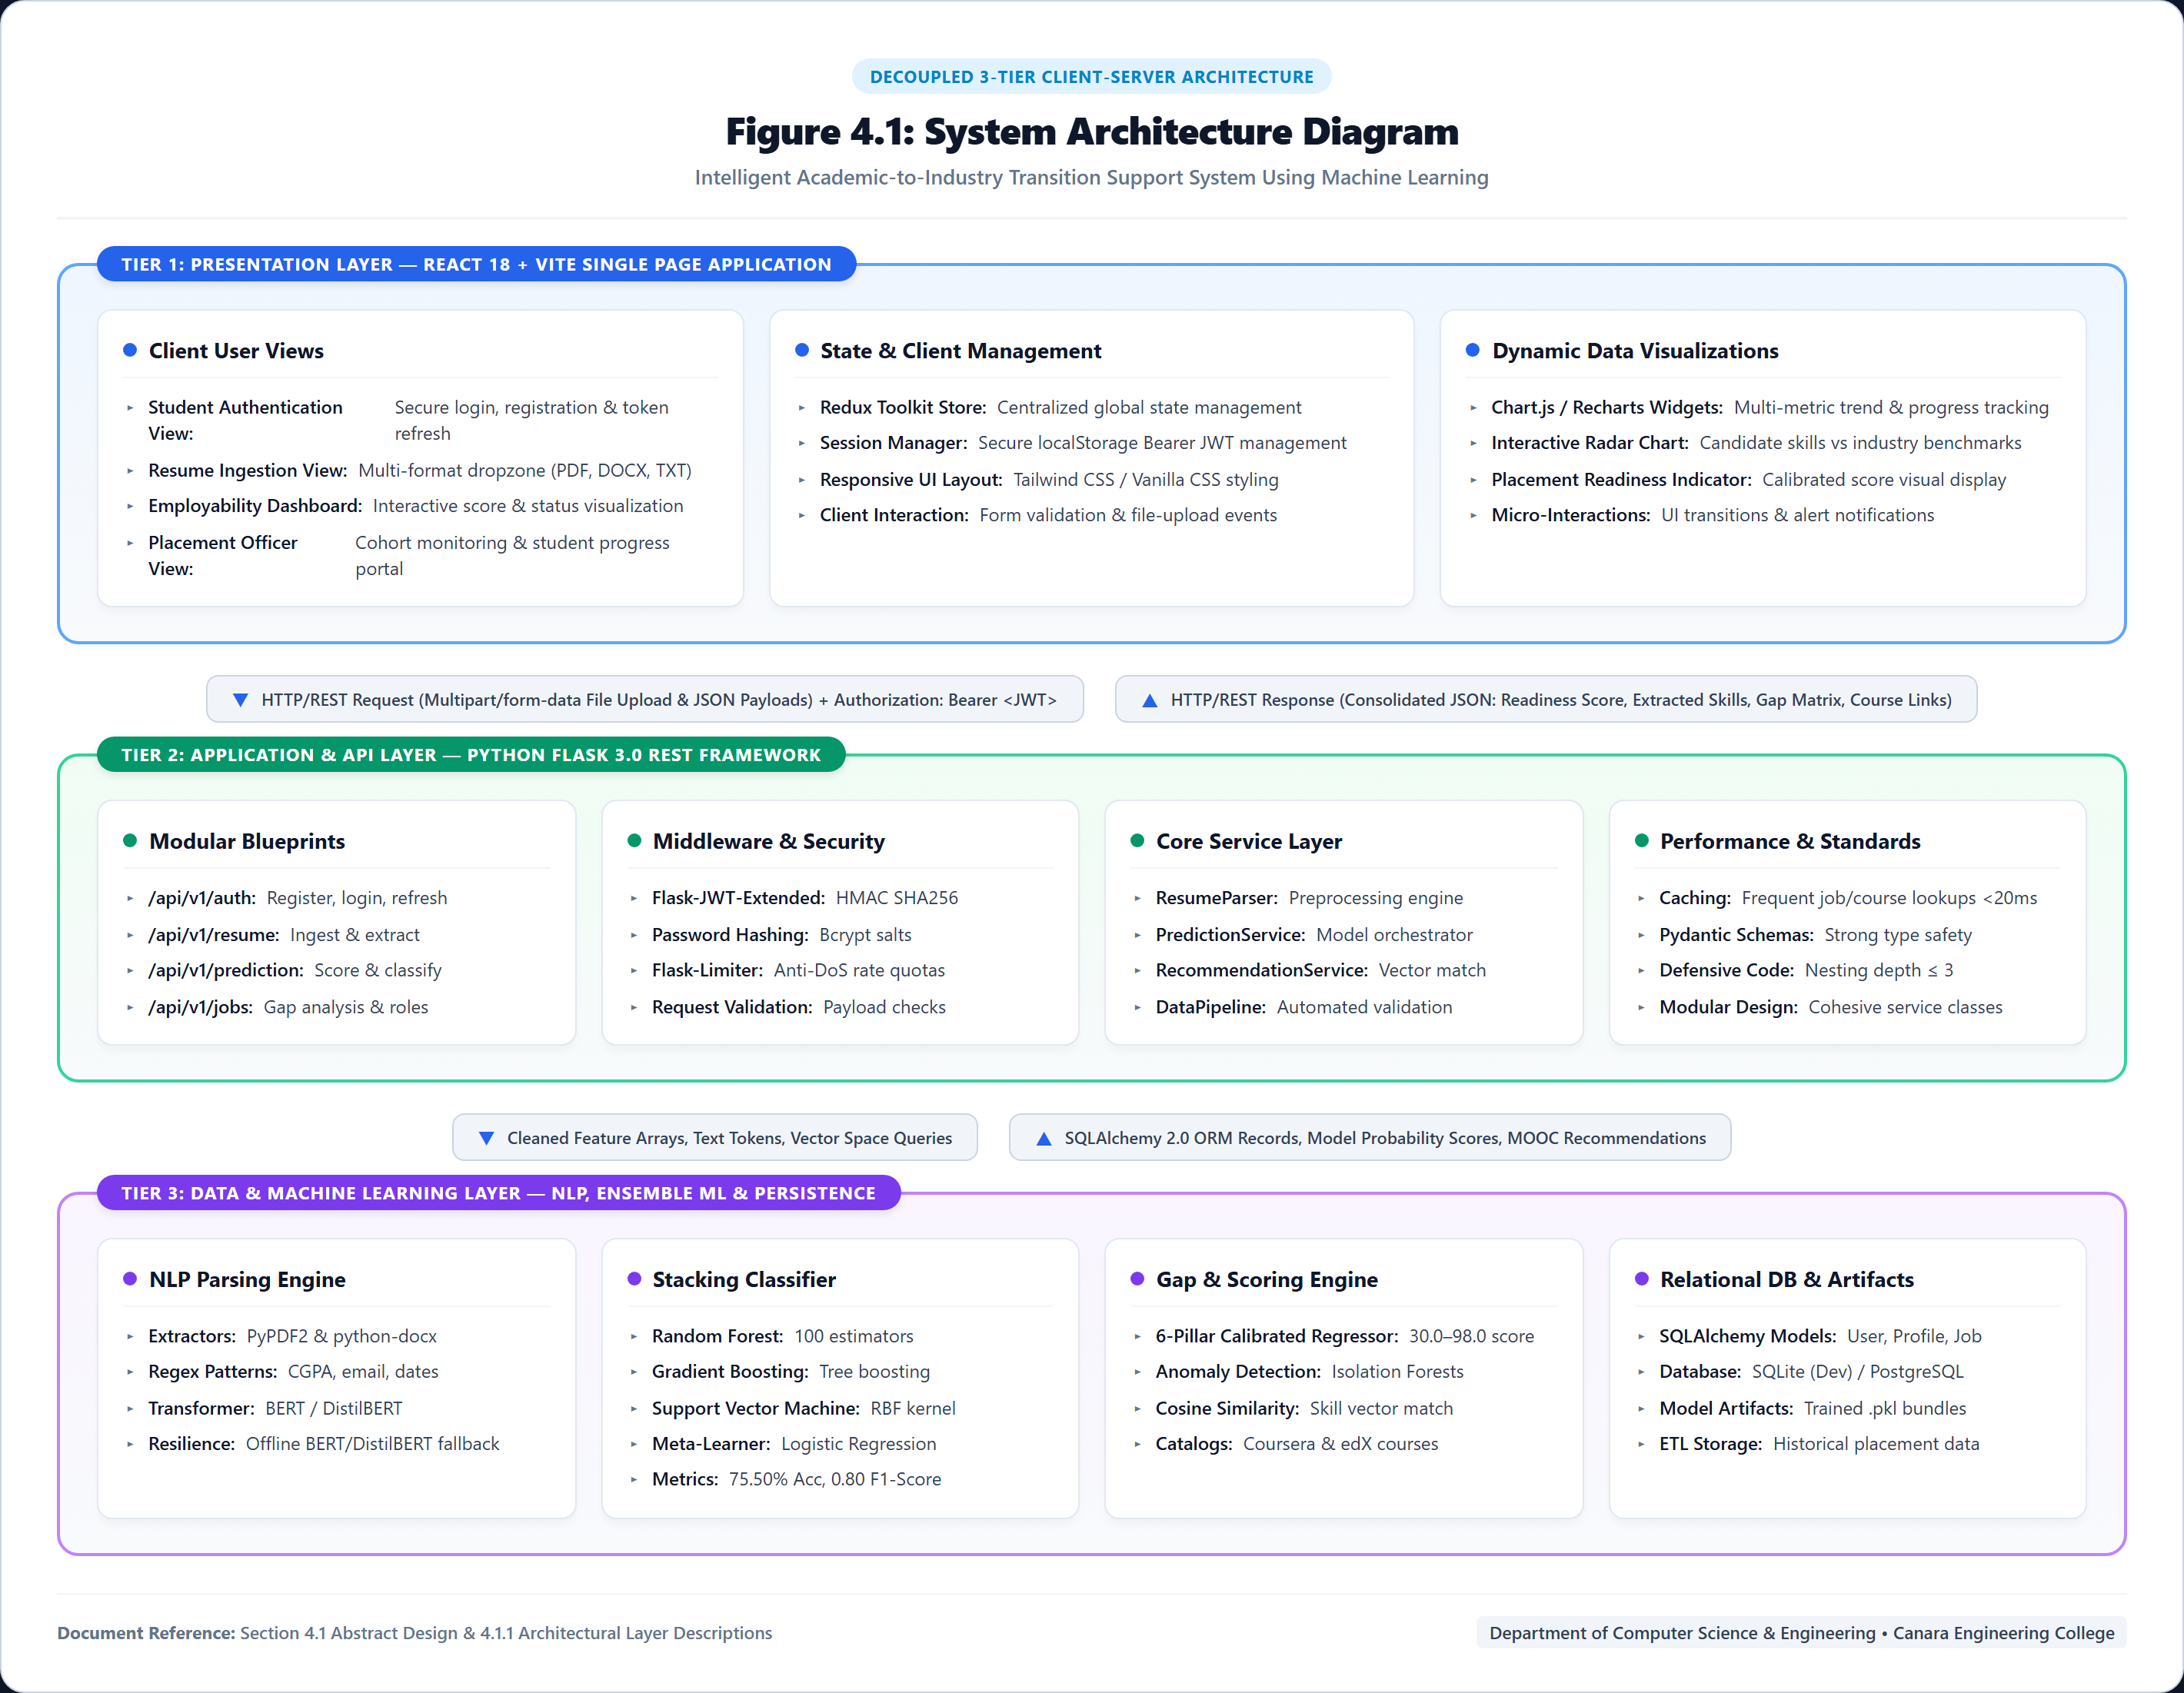
\includegraphics[scale=0.5]{./pic/ar.png}
\caption{System Architecture Diagram}
\label{fig:arch}
\end{figure}

\subsection{Architectural Layer Descriptions}
\begin{enumerate}
    \item \textbf{Presentation Layer (Frontend)}: Built with React 18 and Vite, managing user interactions, authentication state, file upload events, and dynamic Chart.js/Recharts data visualizations.
    \item \textbf{Application Layer (Flask REST API)}: Modular Flask Blueprints handling route dispatching, JWT authorization, rate limiting, request validation, and orchestrating service calls.
    \item \textbf{Data \& Intelligence Layer}: Houses the NLP parsing engine, Stacking Ensemble classifier, five-pillar calibrated regressor, Vector Space recommendation engine, and relational databases.
\end{enumerate}

\section{Proposed System Flow}
The end-to-end procedural flow of the proposed transition support platform is illustrated below:

\begin{figure}[htbp]
\centering
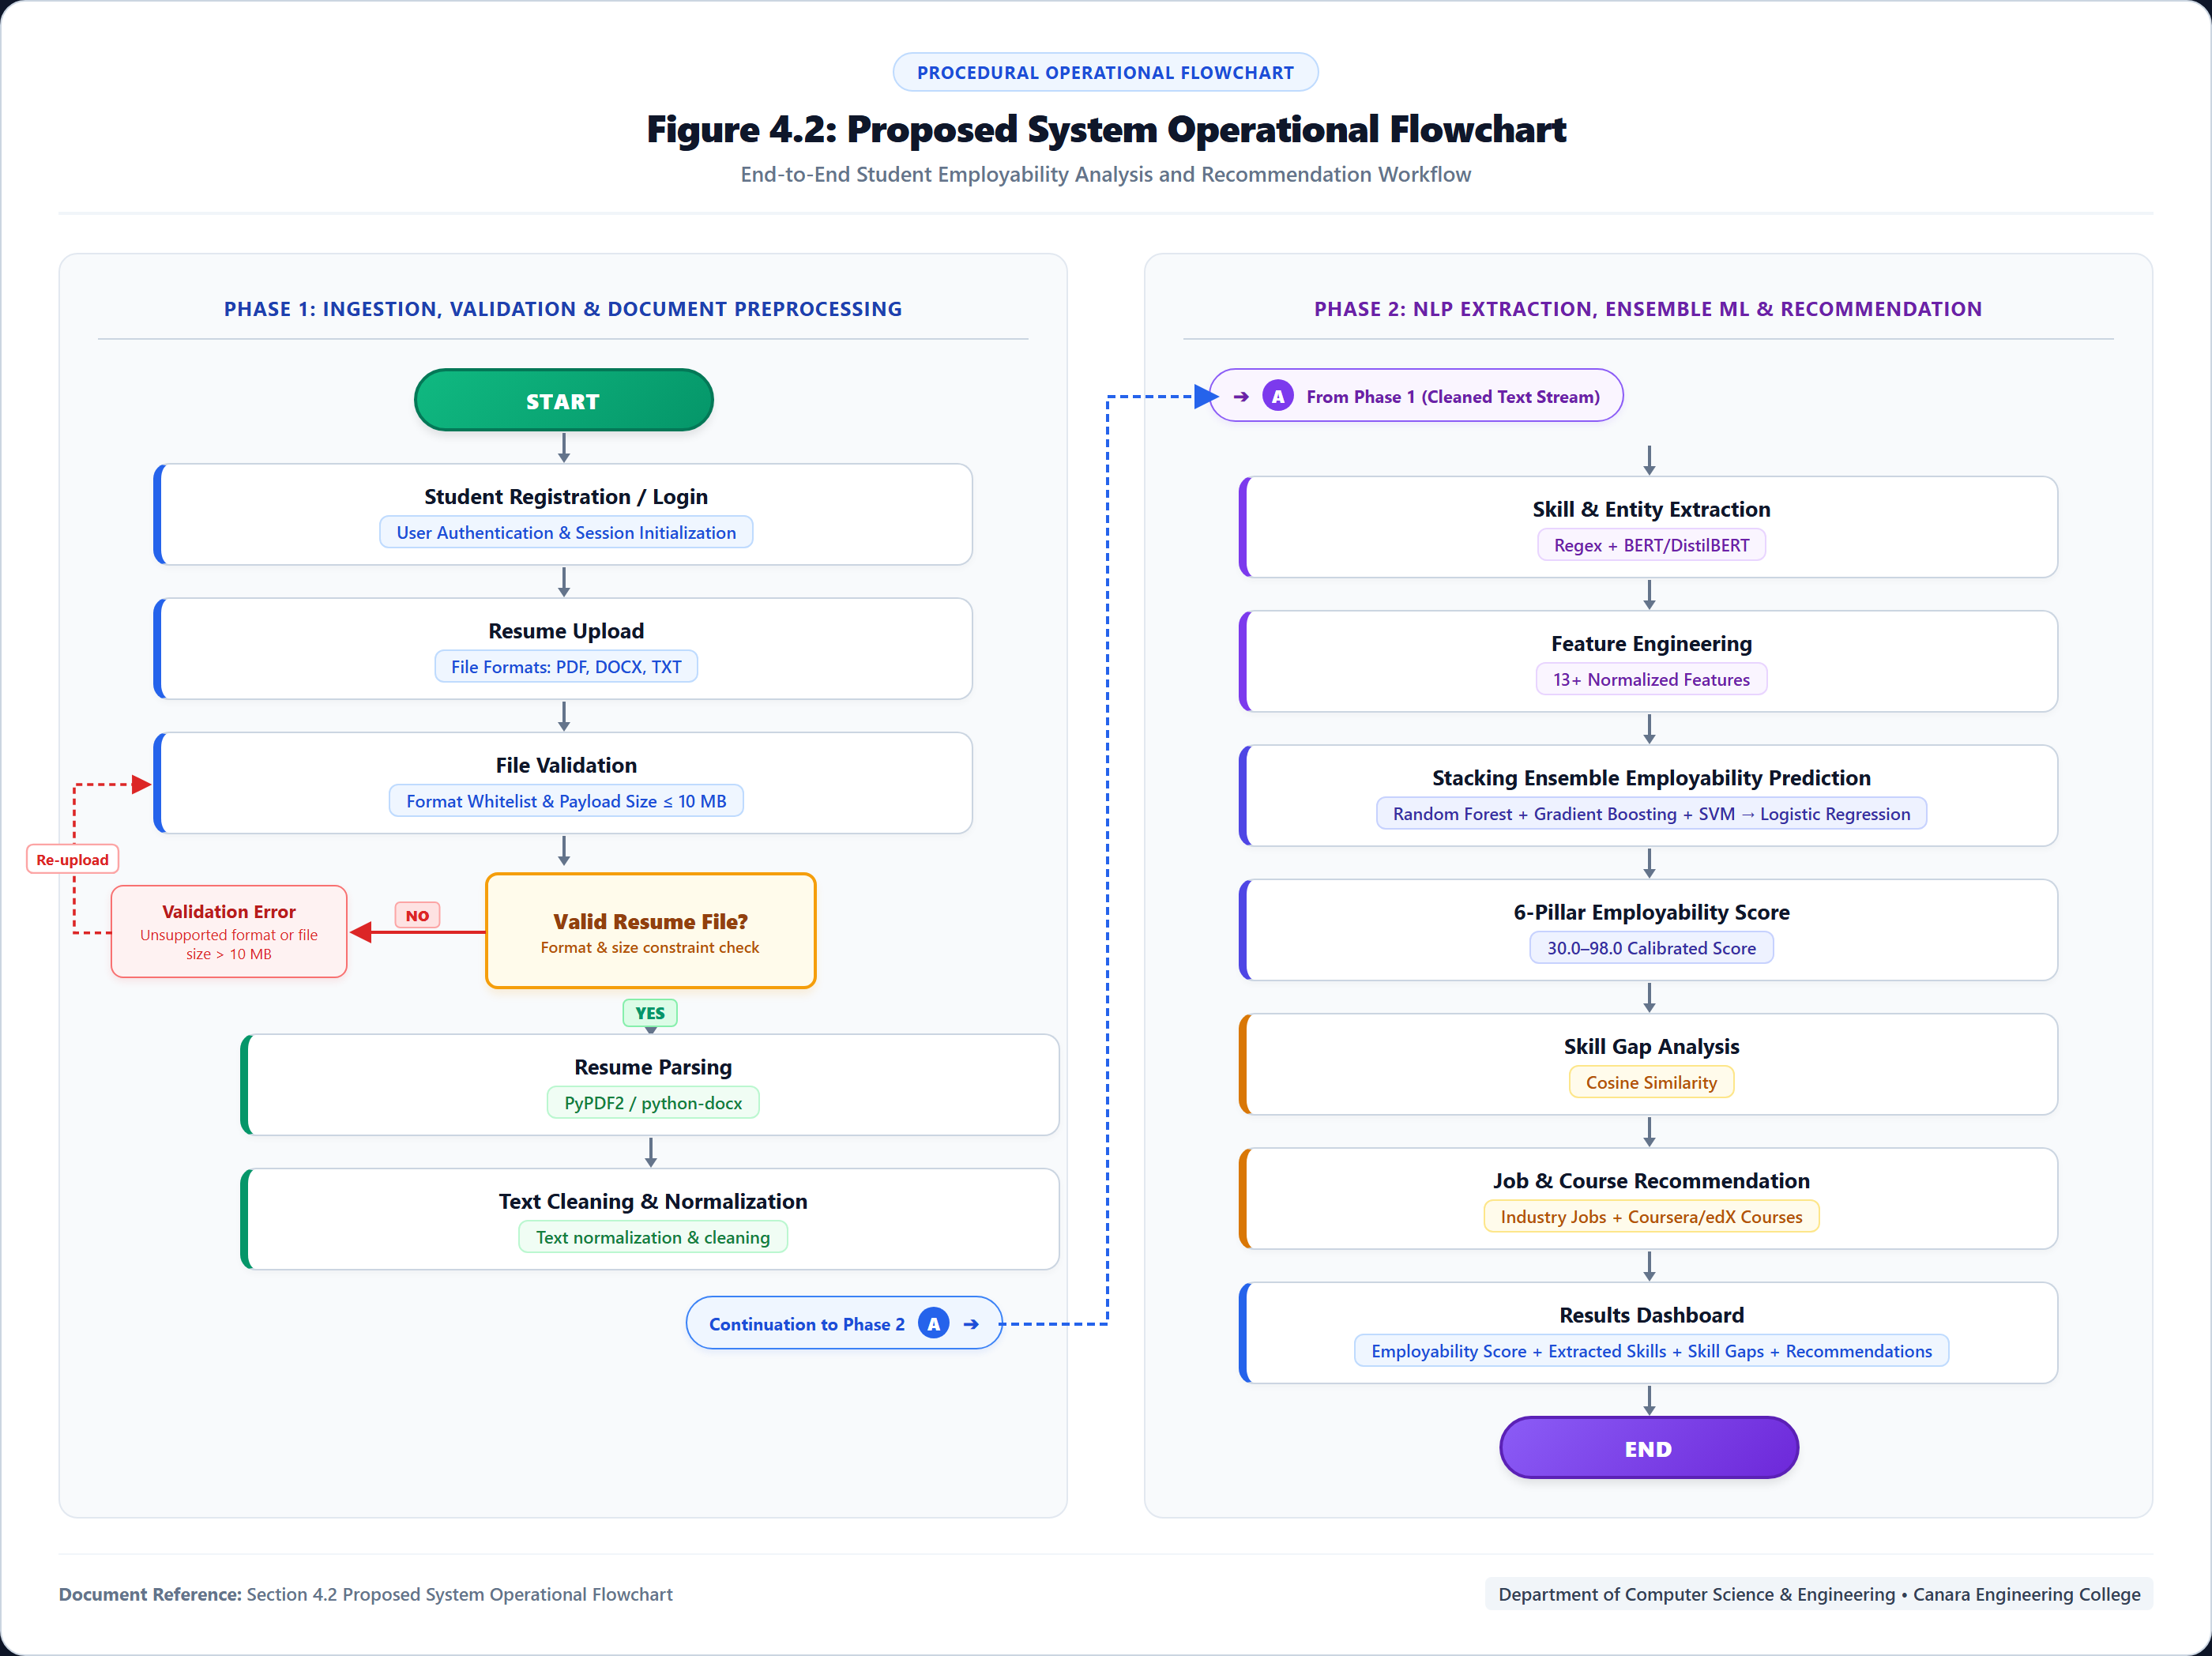
\includegraphics[scale=0.5]{./pic/flowchartforblind.png}
\caption{Proposed System Operational Flowchart}
\label{fig:flowchart}
\end{figure}

\newpage
\section{Functional Design}

\subsection{Modular Design}
The system is partitioned into independent, loosely coupled modules ensuring high cohesion:

\begin{figure}[hbtp]
\centering
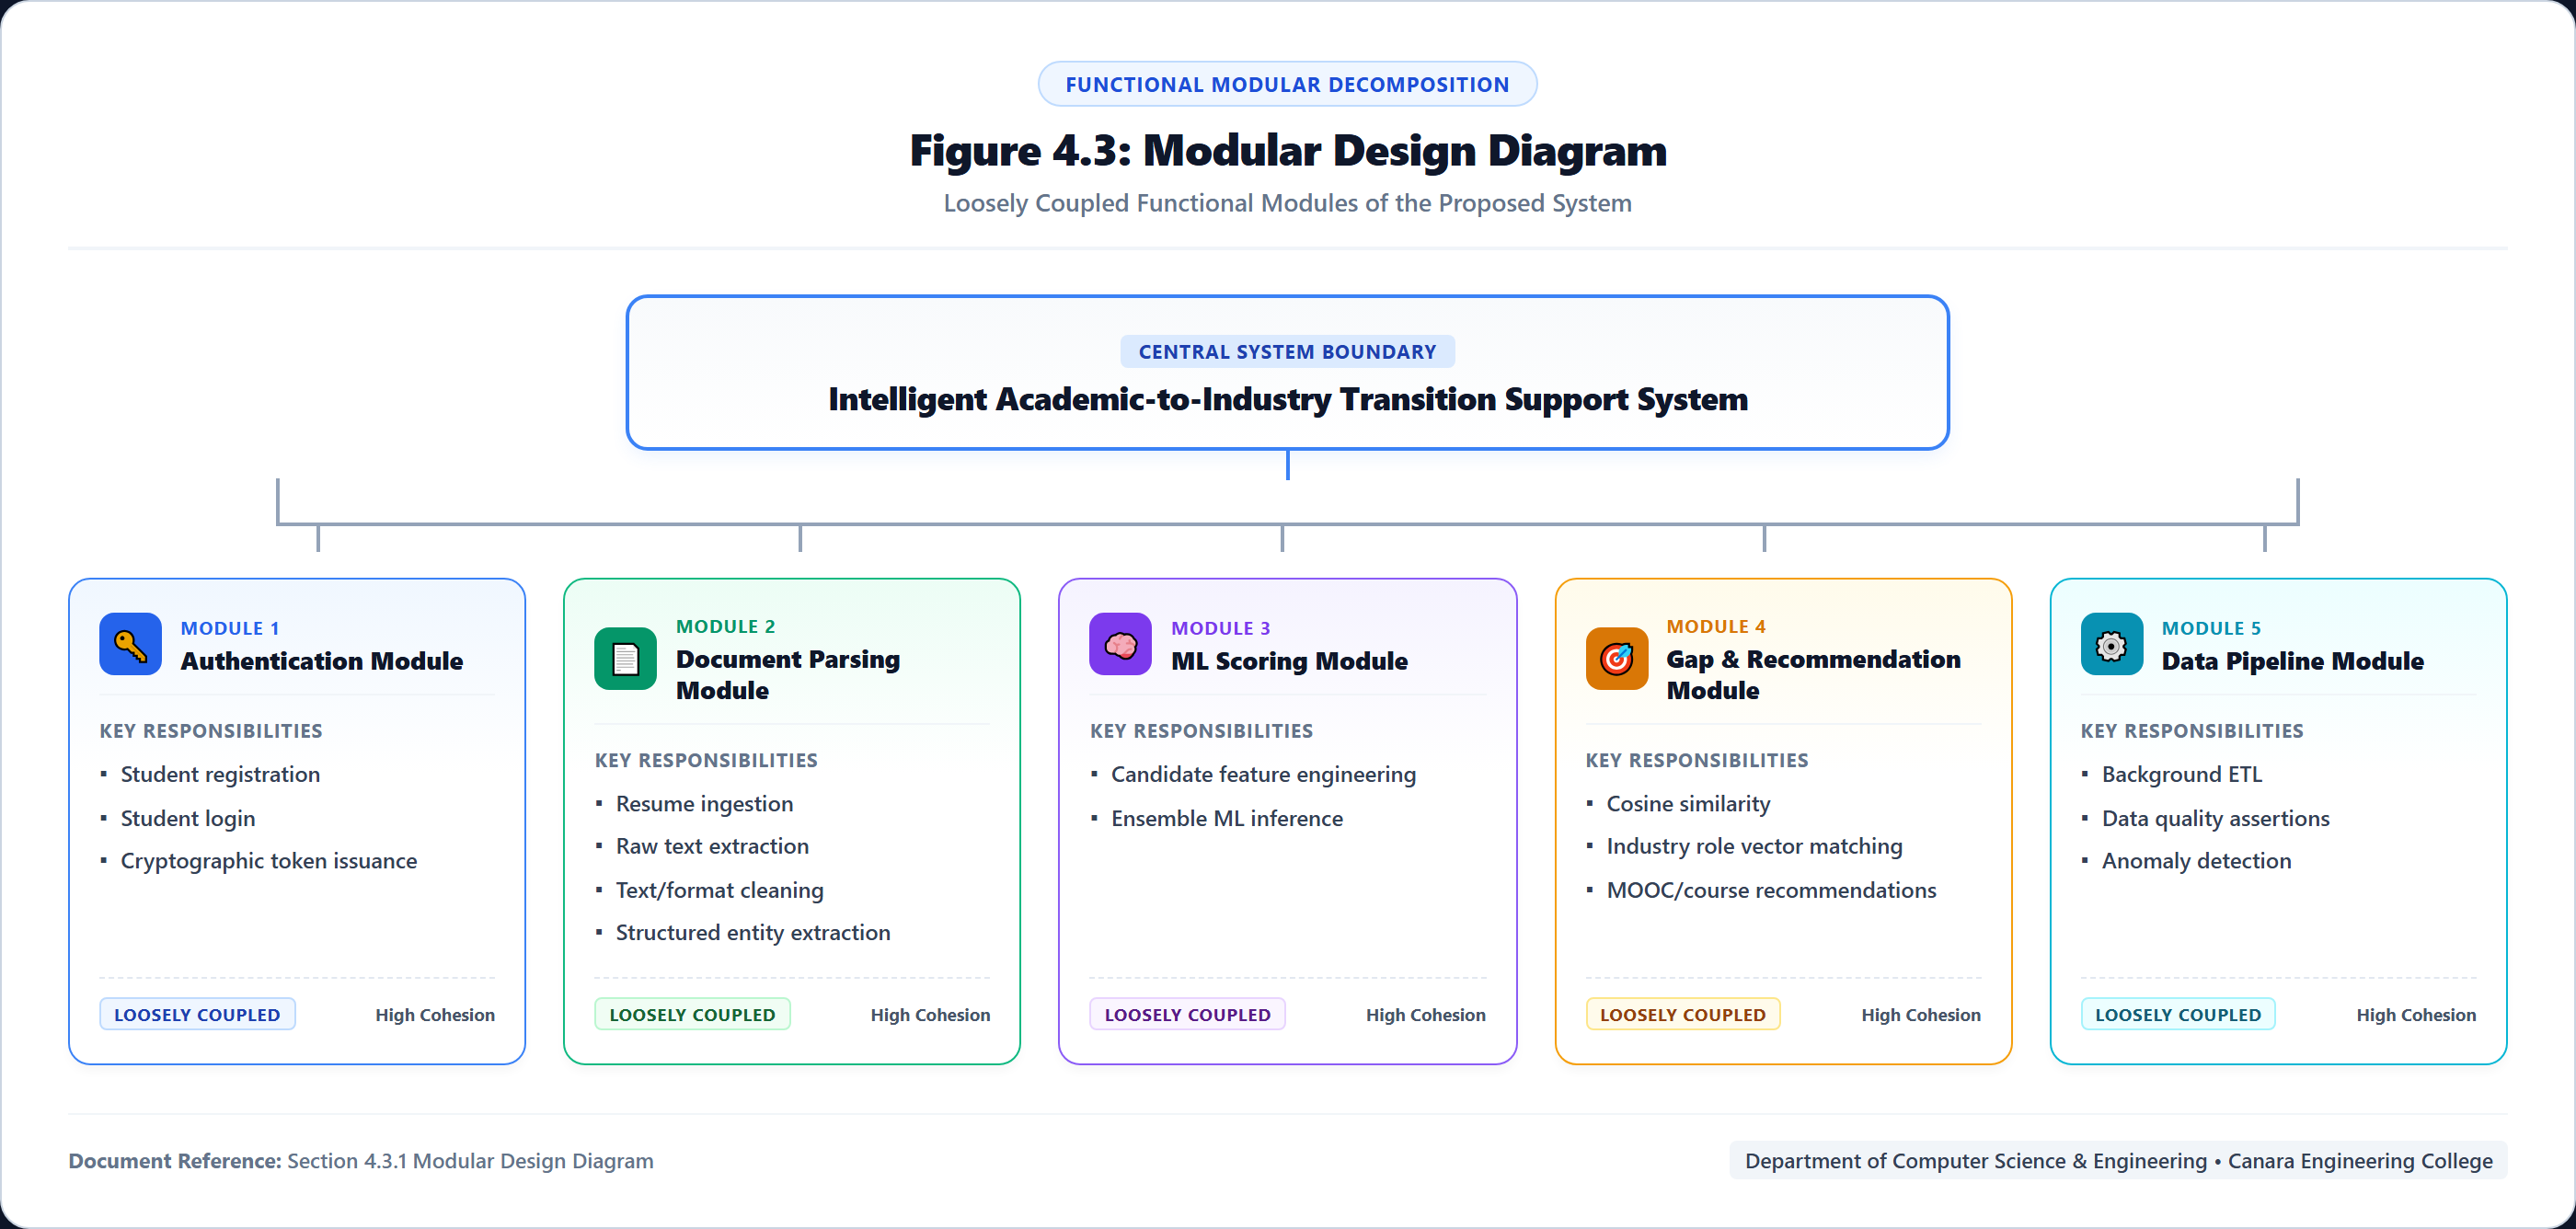
\includegraphics[width=5in,height=3.5in]{./pic/modular.png}
\caption{Modular Design Diagram}
\label{fig:modular}
\end{figure}

\begin{itemize}
    \item \textbf{Authentication Module}: Manages student login, registration, and cryptographic token issuance.
    \item \textbf{Document Parsing Module}: Ingests resumes, extracts raw text, cleans formatting, and isolates structured entities.
    \item \textbf{ML Scoring Module}: Featurizes candidate data and executes ensemble inference.
    \item \textbf{Gap \& Recommendation Module}: Computes cosine similarity against industry role vectors and MOOC databases.
    \item \textbf{Data Pipeline Module}: Performs background ETL, data quality assertion, and anomaly detection.
\end{itemize}

\newpage
\subsection{Sequence Diagram}
The sequence diagram models the chronological interaction between system entities during a typical analysis cycle:

\begin{figure}[hbtp]
\centering
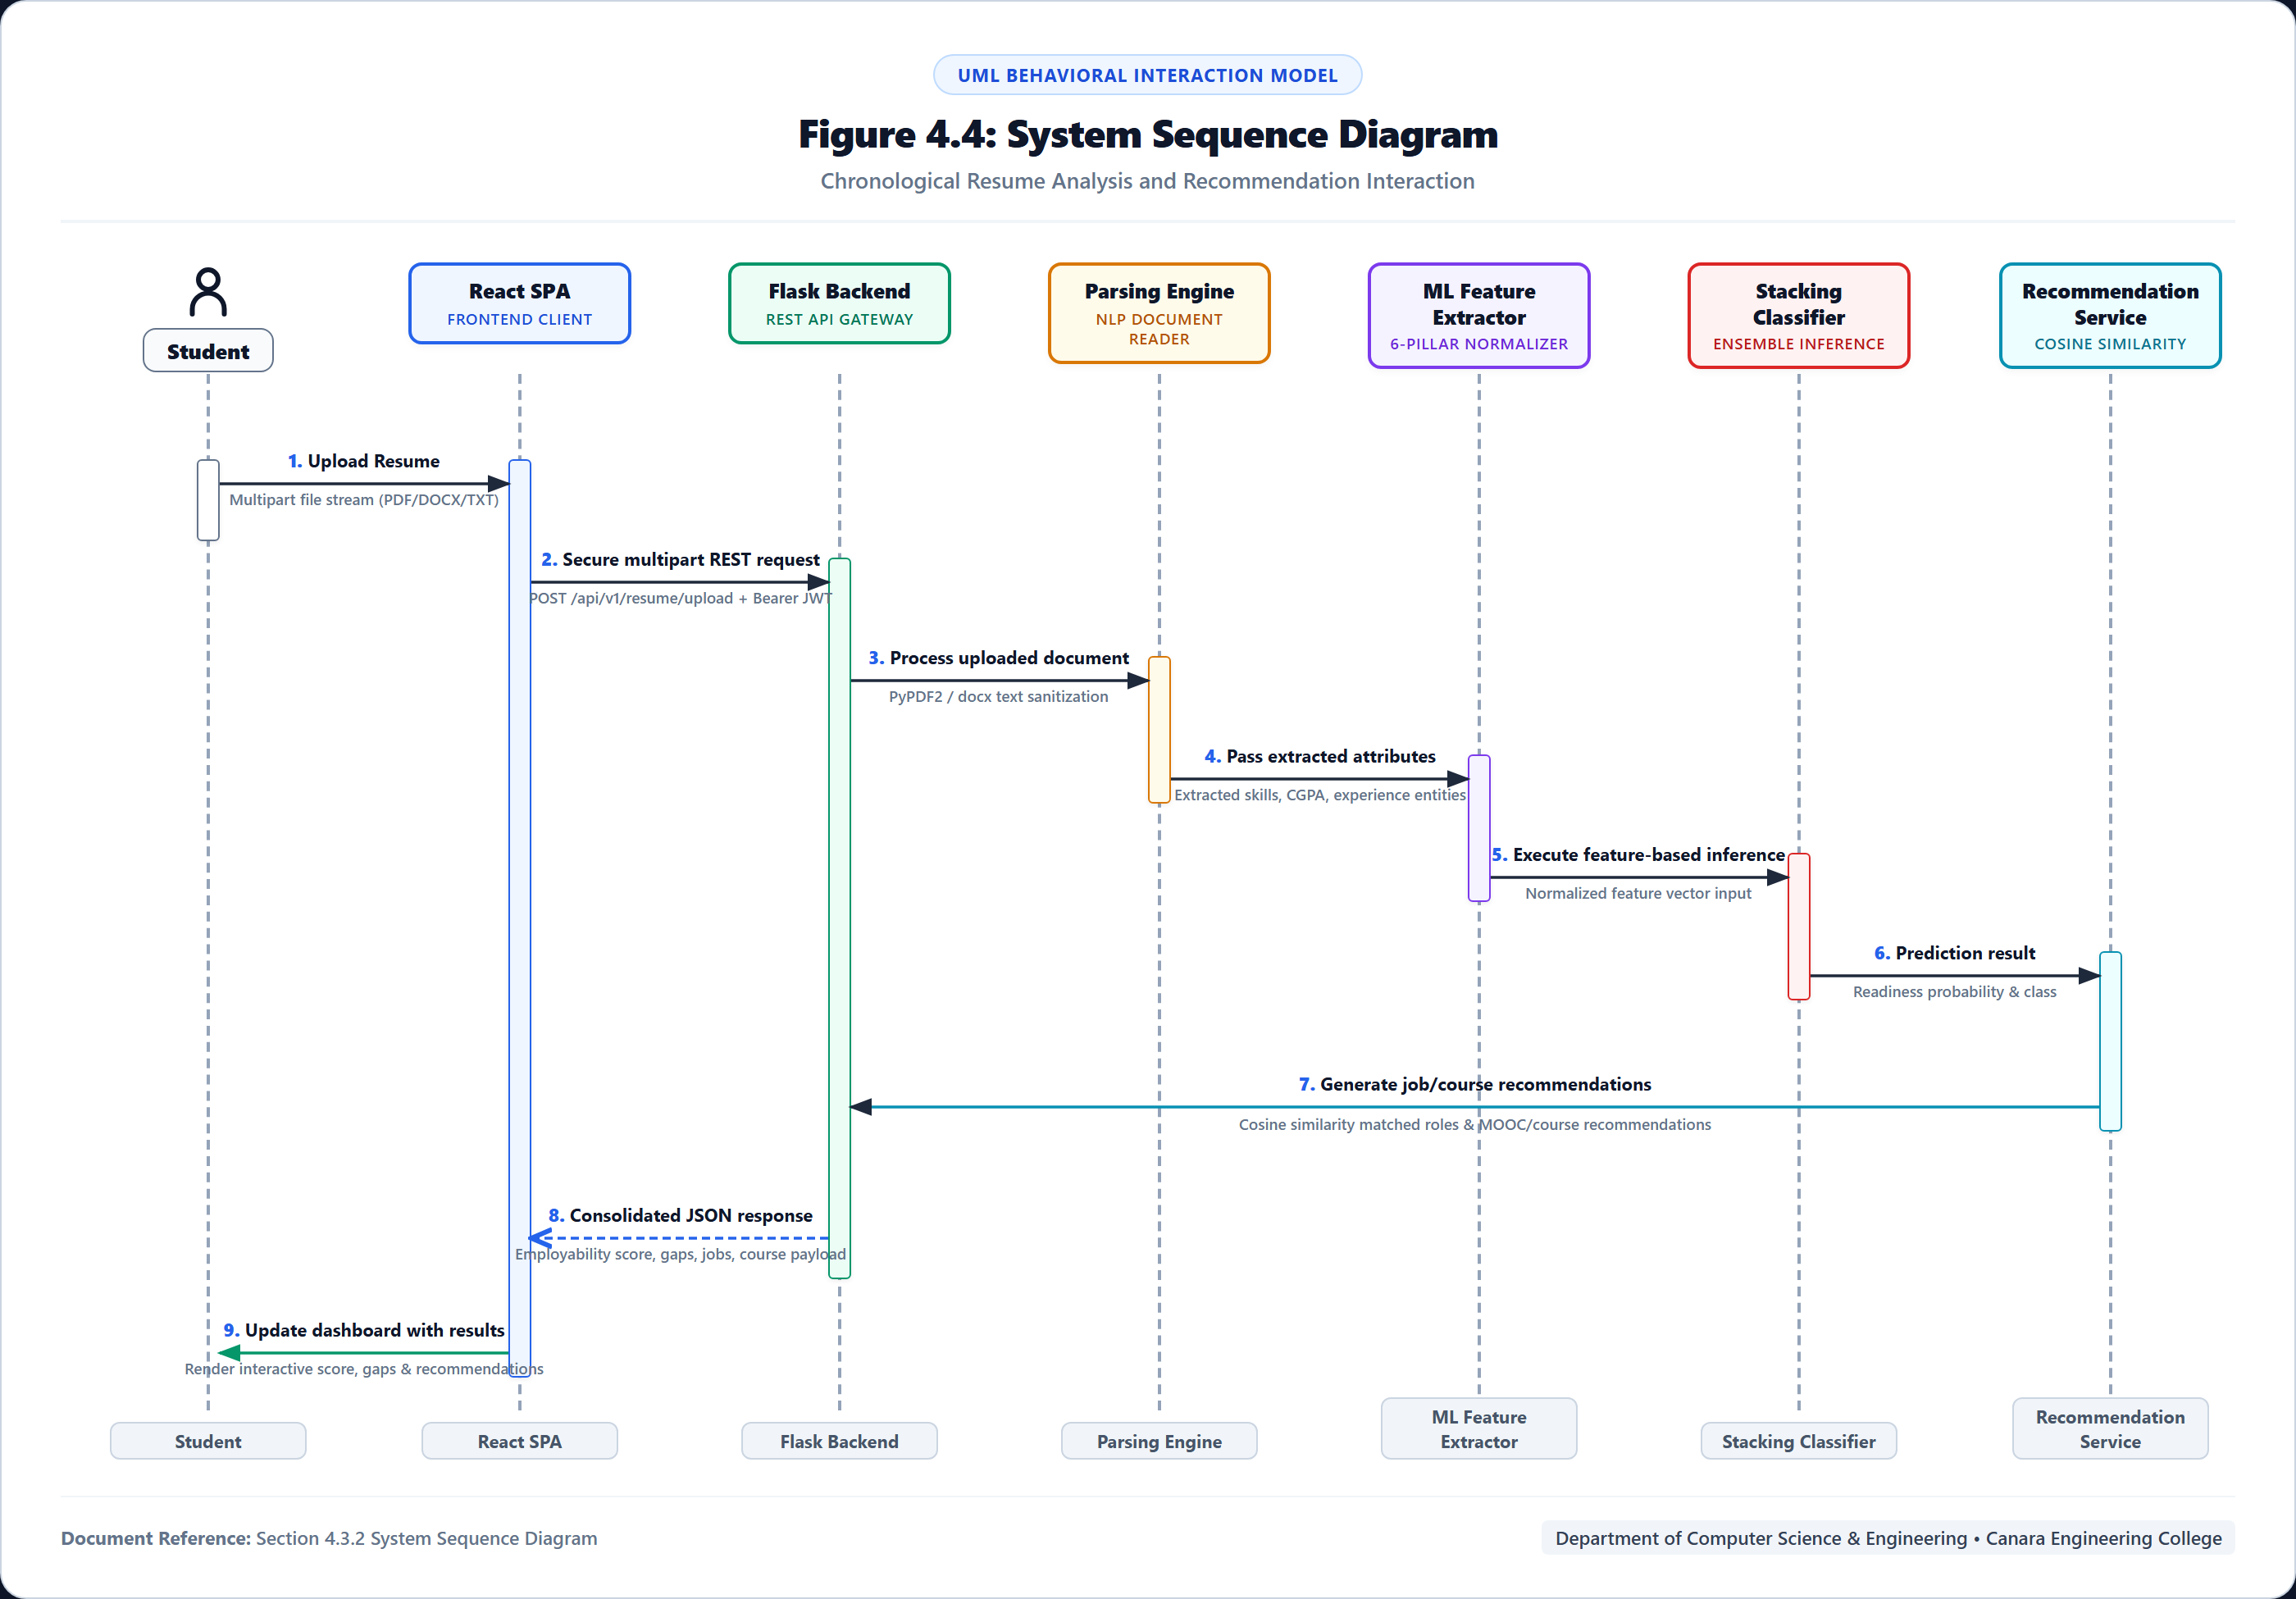
\includegraphics[width=5.2in,height=4.2in]{./pic/sequence.png}
\caption{System Sequence Diagram}
\label{fig:sequence}
\end{figure}

\par As shown, the student uploads their resume through the React SPA. The file is transmitted via a secure multipart REST request to the Flask backend. The parsing engine processes the document, passes extracted attributes to the ML feature extractor, executes Stacking Classifier inference, and generates job/course recommendations before returning a consolidated JSON response to update the frontend dashboard.

\newpage
\subsection{Use Case Diagram}
The use case diagram illustrates user and administrator interactions with the system:

\begin{figure}[hbtp]
\centering
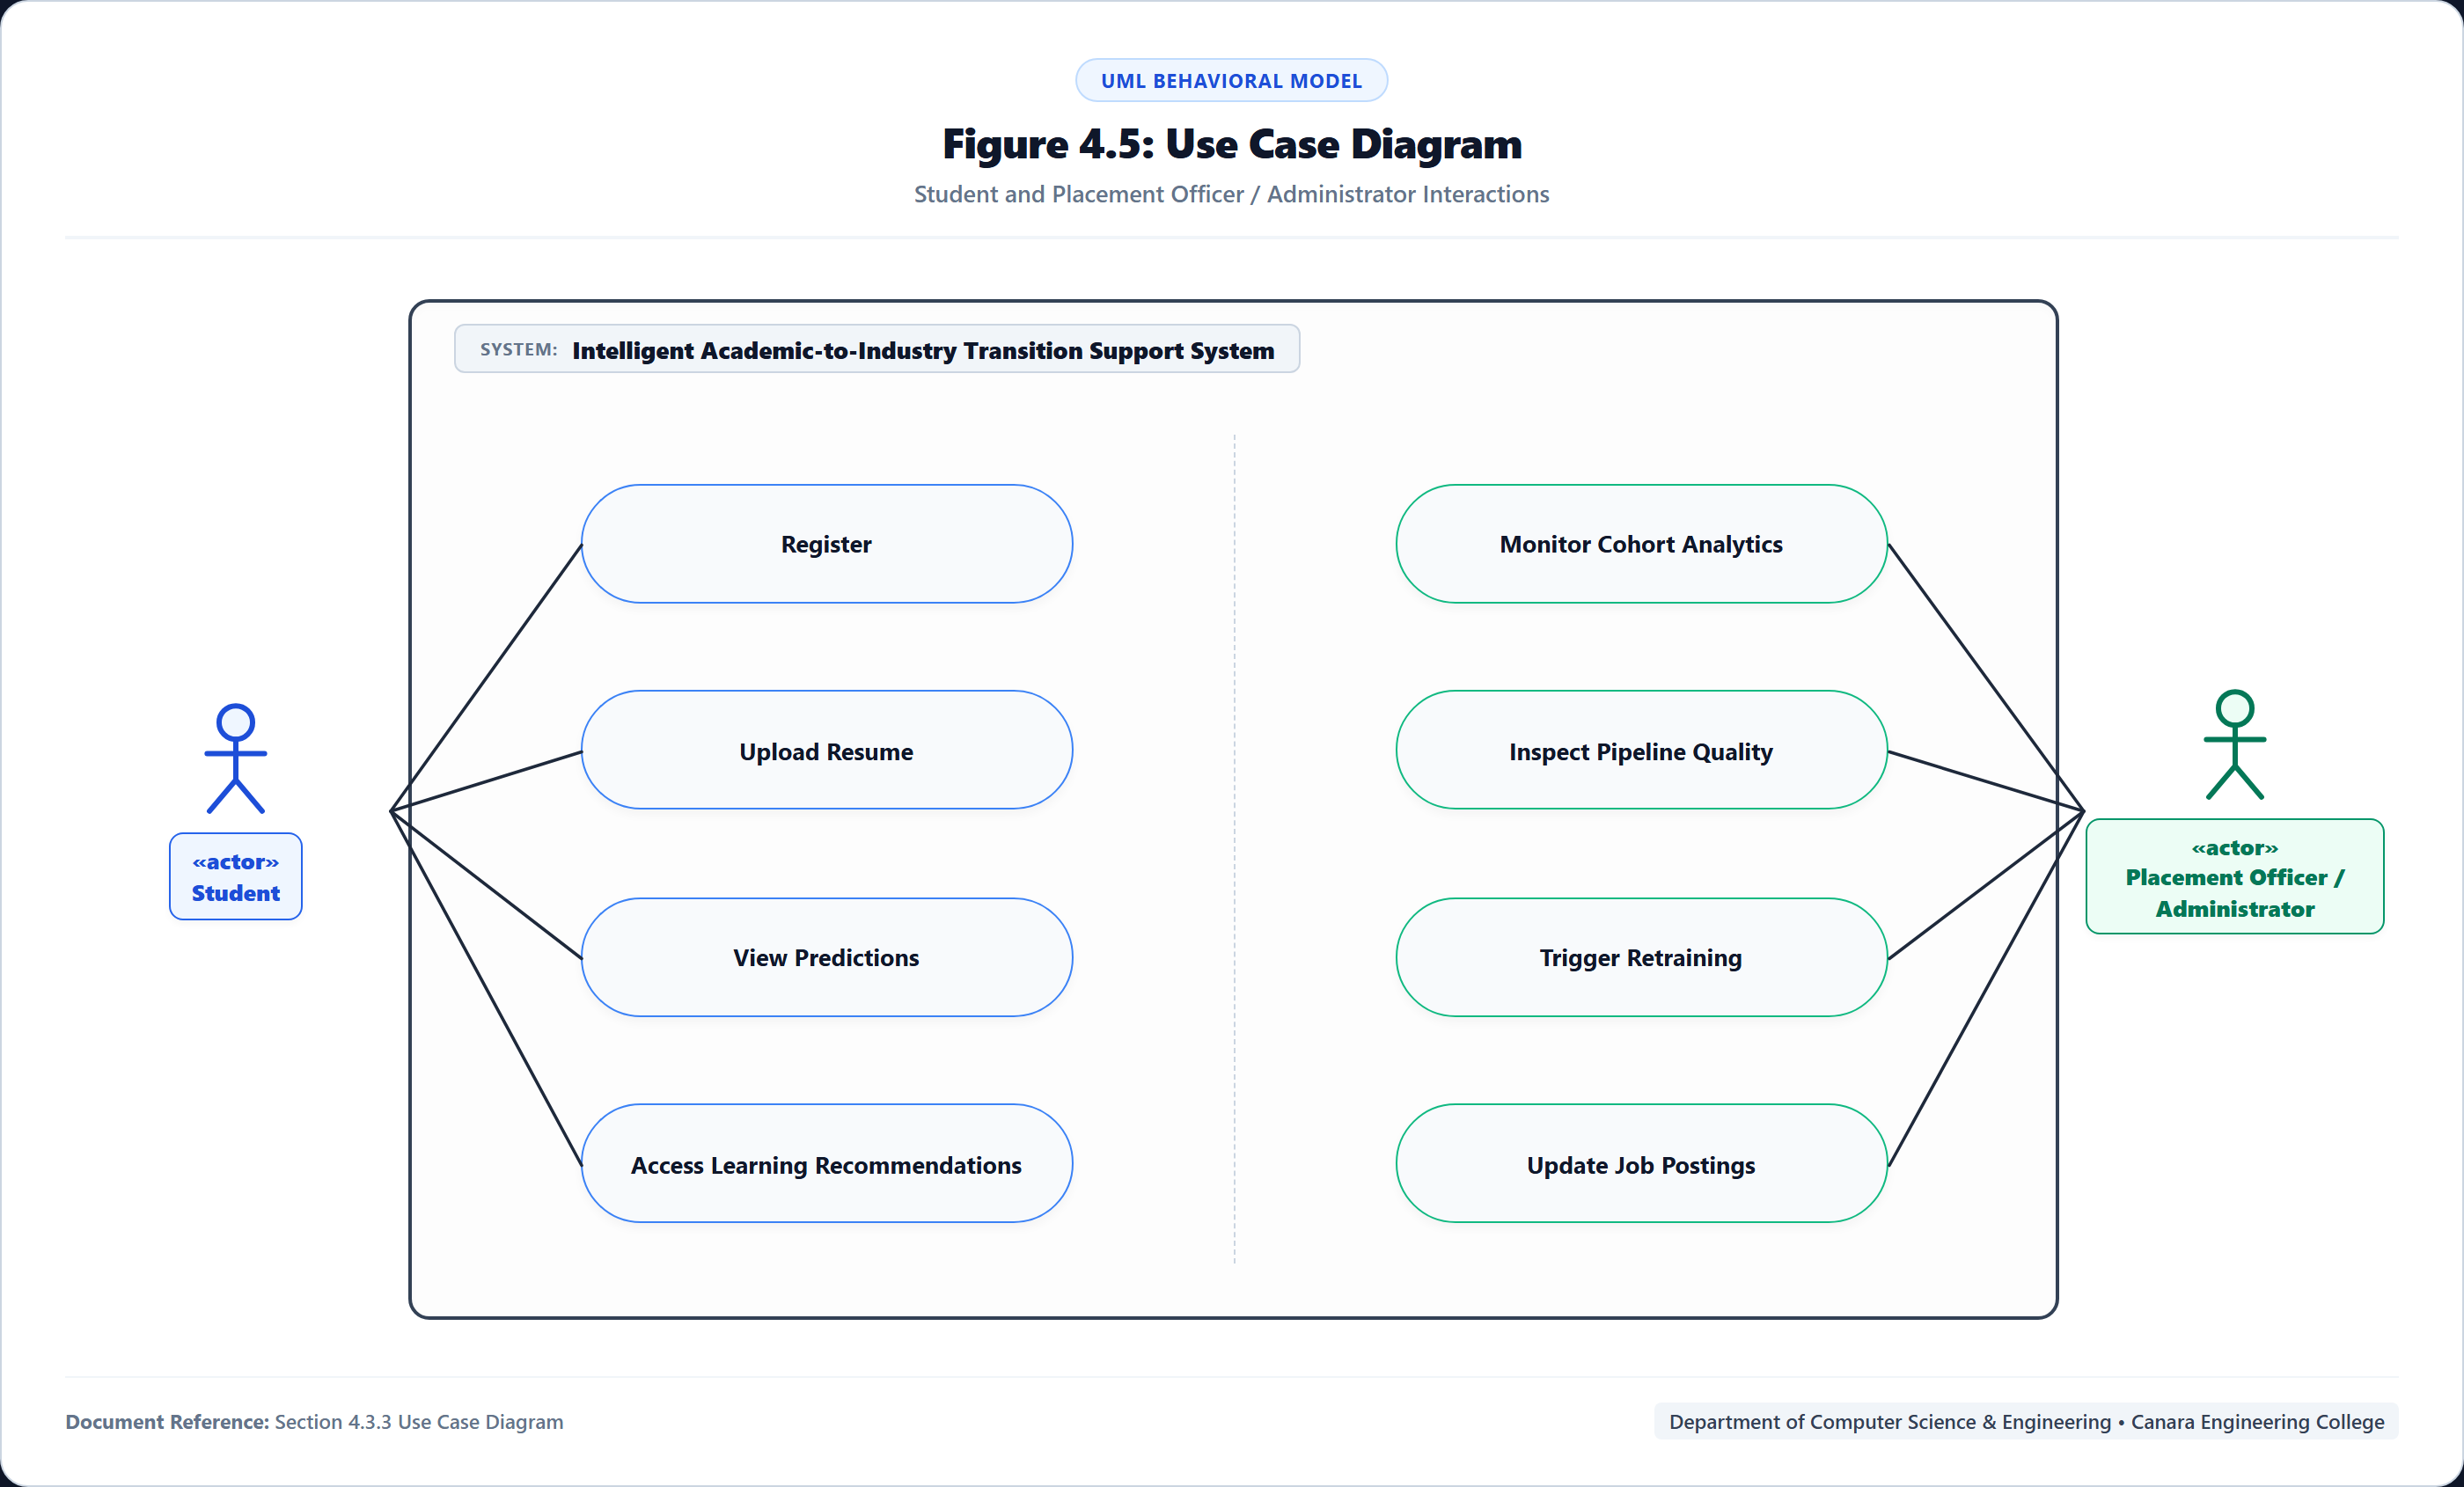
\includegraphics[width=5in,height=4.5in]{./pic/usecase.png}
\caption{Use Case Diagram}
\label{fig:usecase}
\end{figure}

\par Primary actors include the \textbf{Student} (who registers, uploads resumes, views predictions, and accesses learning recommendations) and the \textbf{Placement Officer / Administrator} (who monitors cohort analytics, inspects pipeline quality, triggers retraining, and updates job postings).

\newpage
\section{Control Flow Design}

\subsection{Activity Diagram}
The activity diagram depicts the conditional execution path followed during resume evaluation and recommendation:

\begin{figure}[hbtp]
\centering
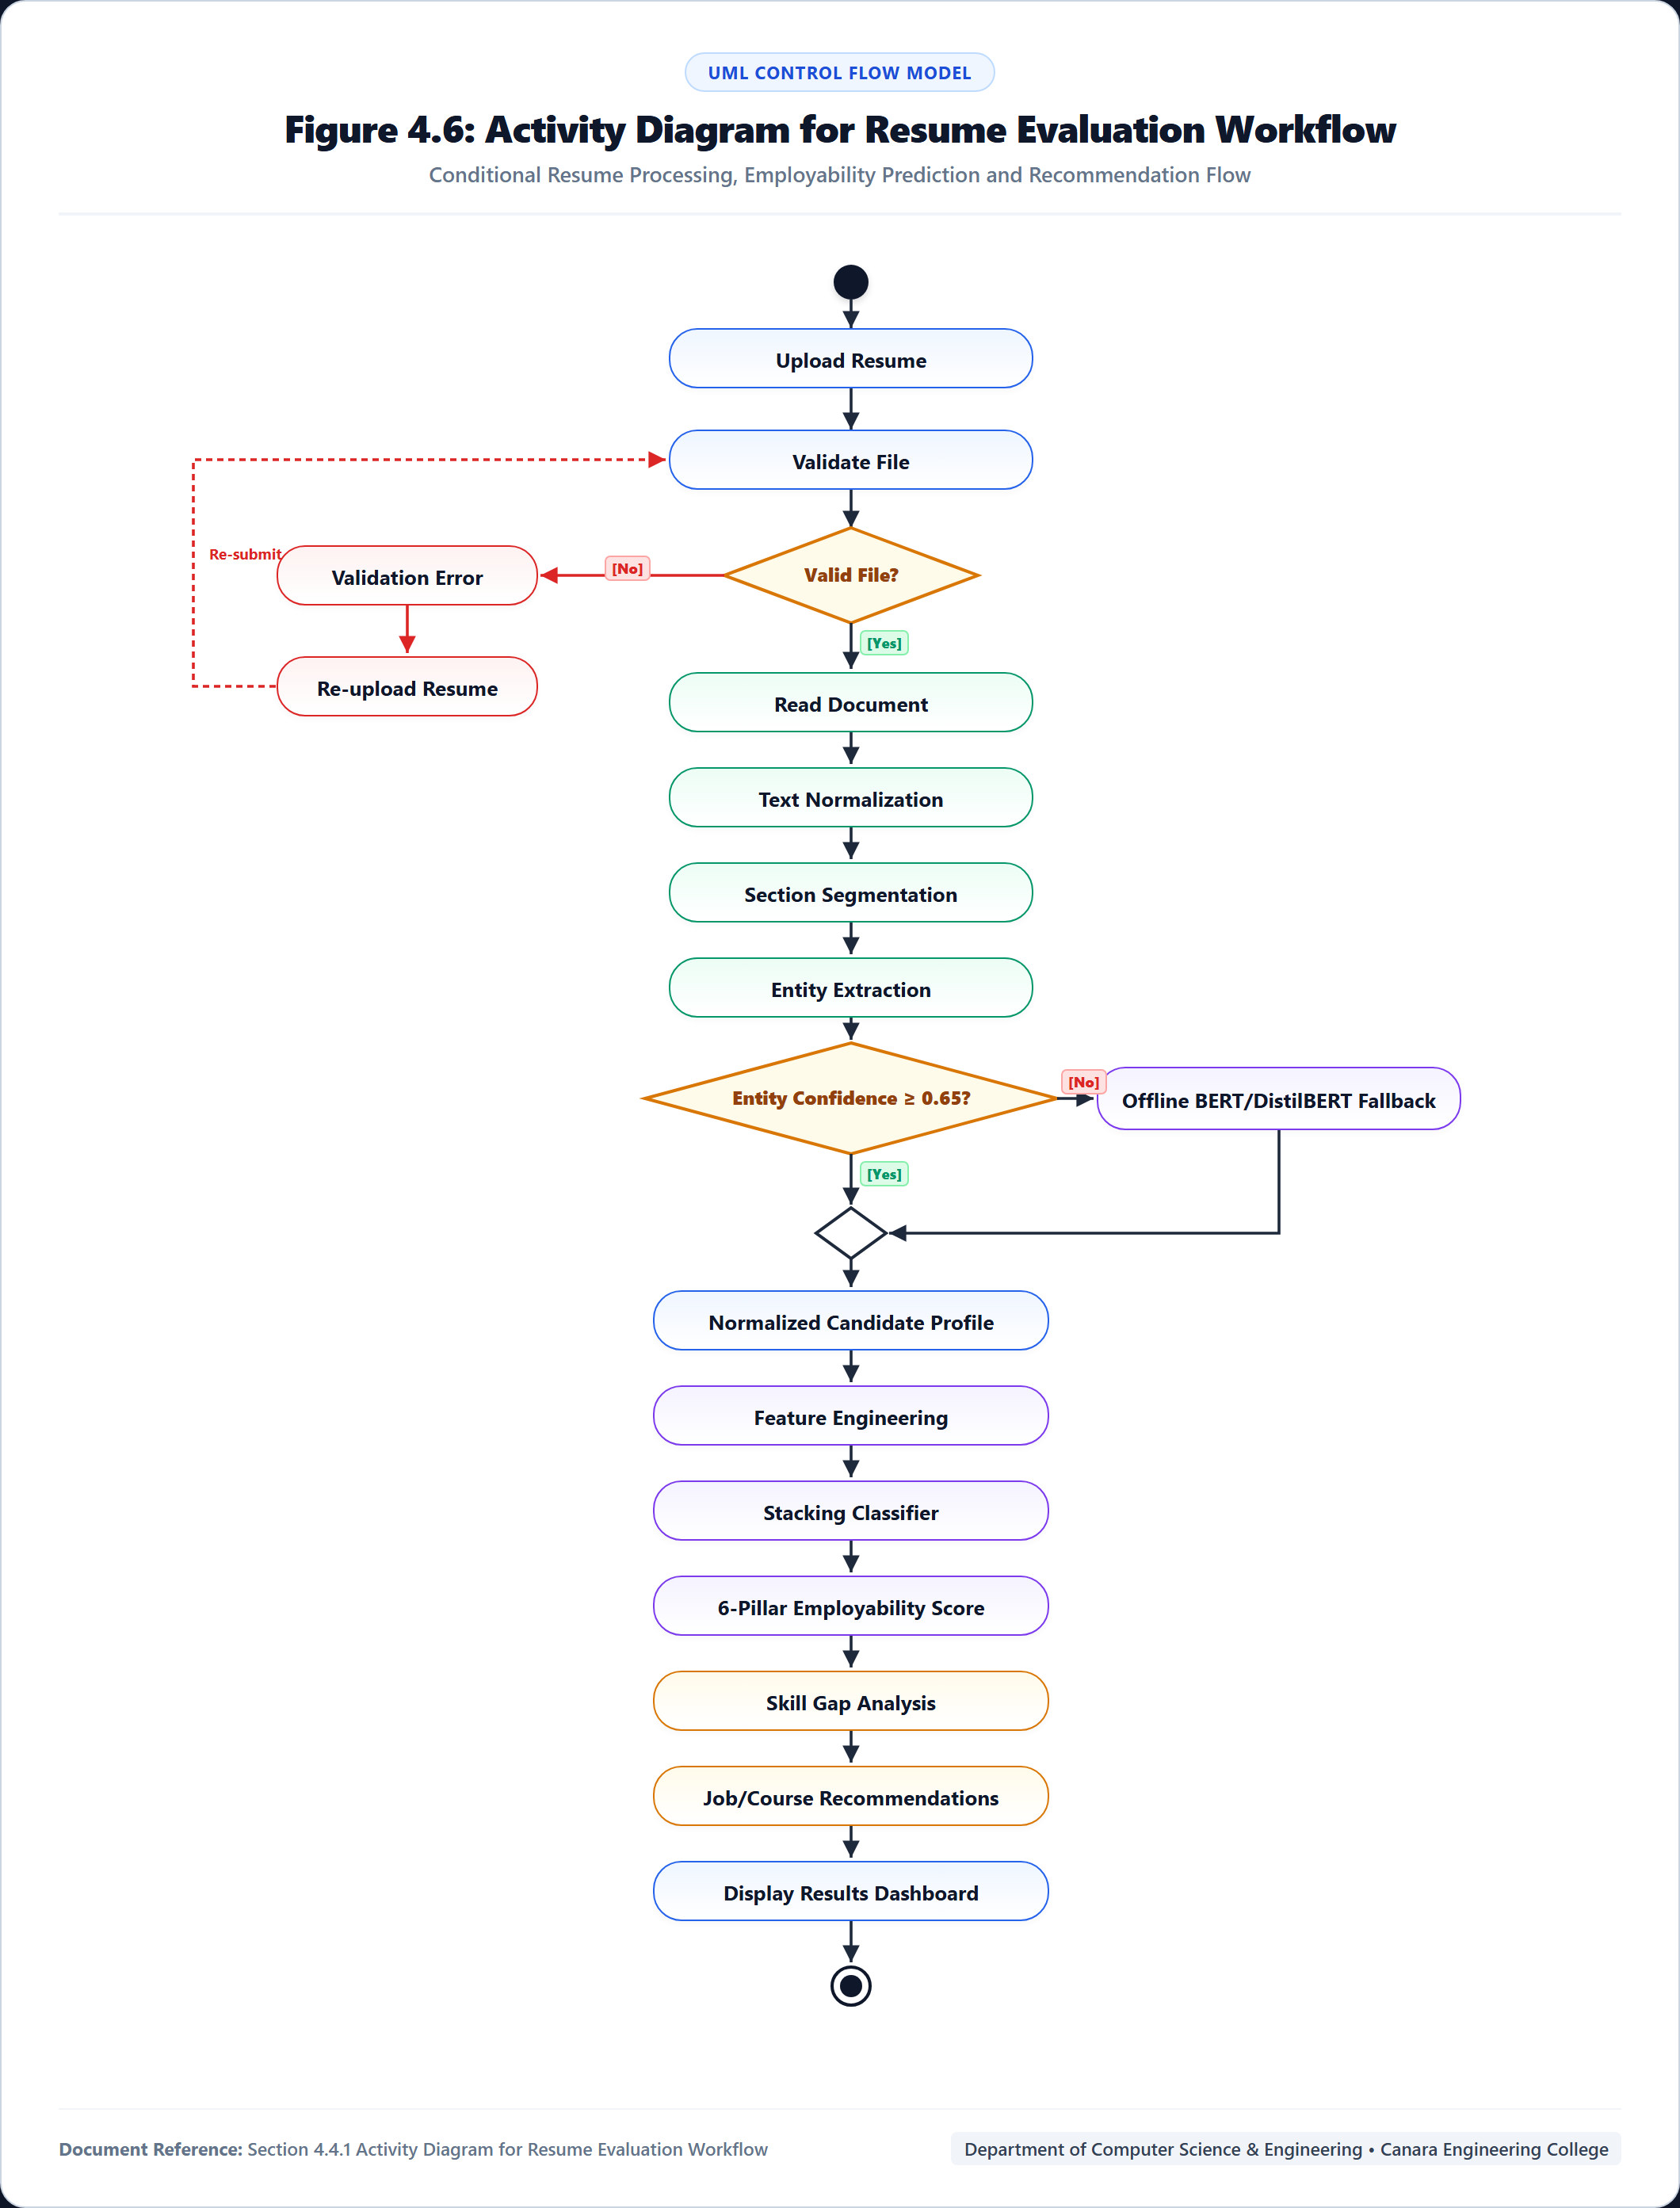
\includegraphics[width=4.8in,height=4.8in]{./pic/activity.png}
\caption{Activity Diagram for Resume Evaluation Workflow}
\label{fig:activity}
\end{figure}

\newpage
\section{Data Flow Design}

\subsection{Zero-Level Data Flow Diagram (Level 0 DFD)}
The Level 0 DFD captures the high-level contextual boundary of the system:

\begin{figure}[hbtp]
\centering
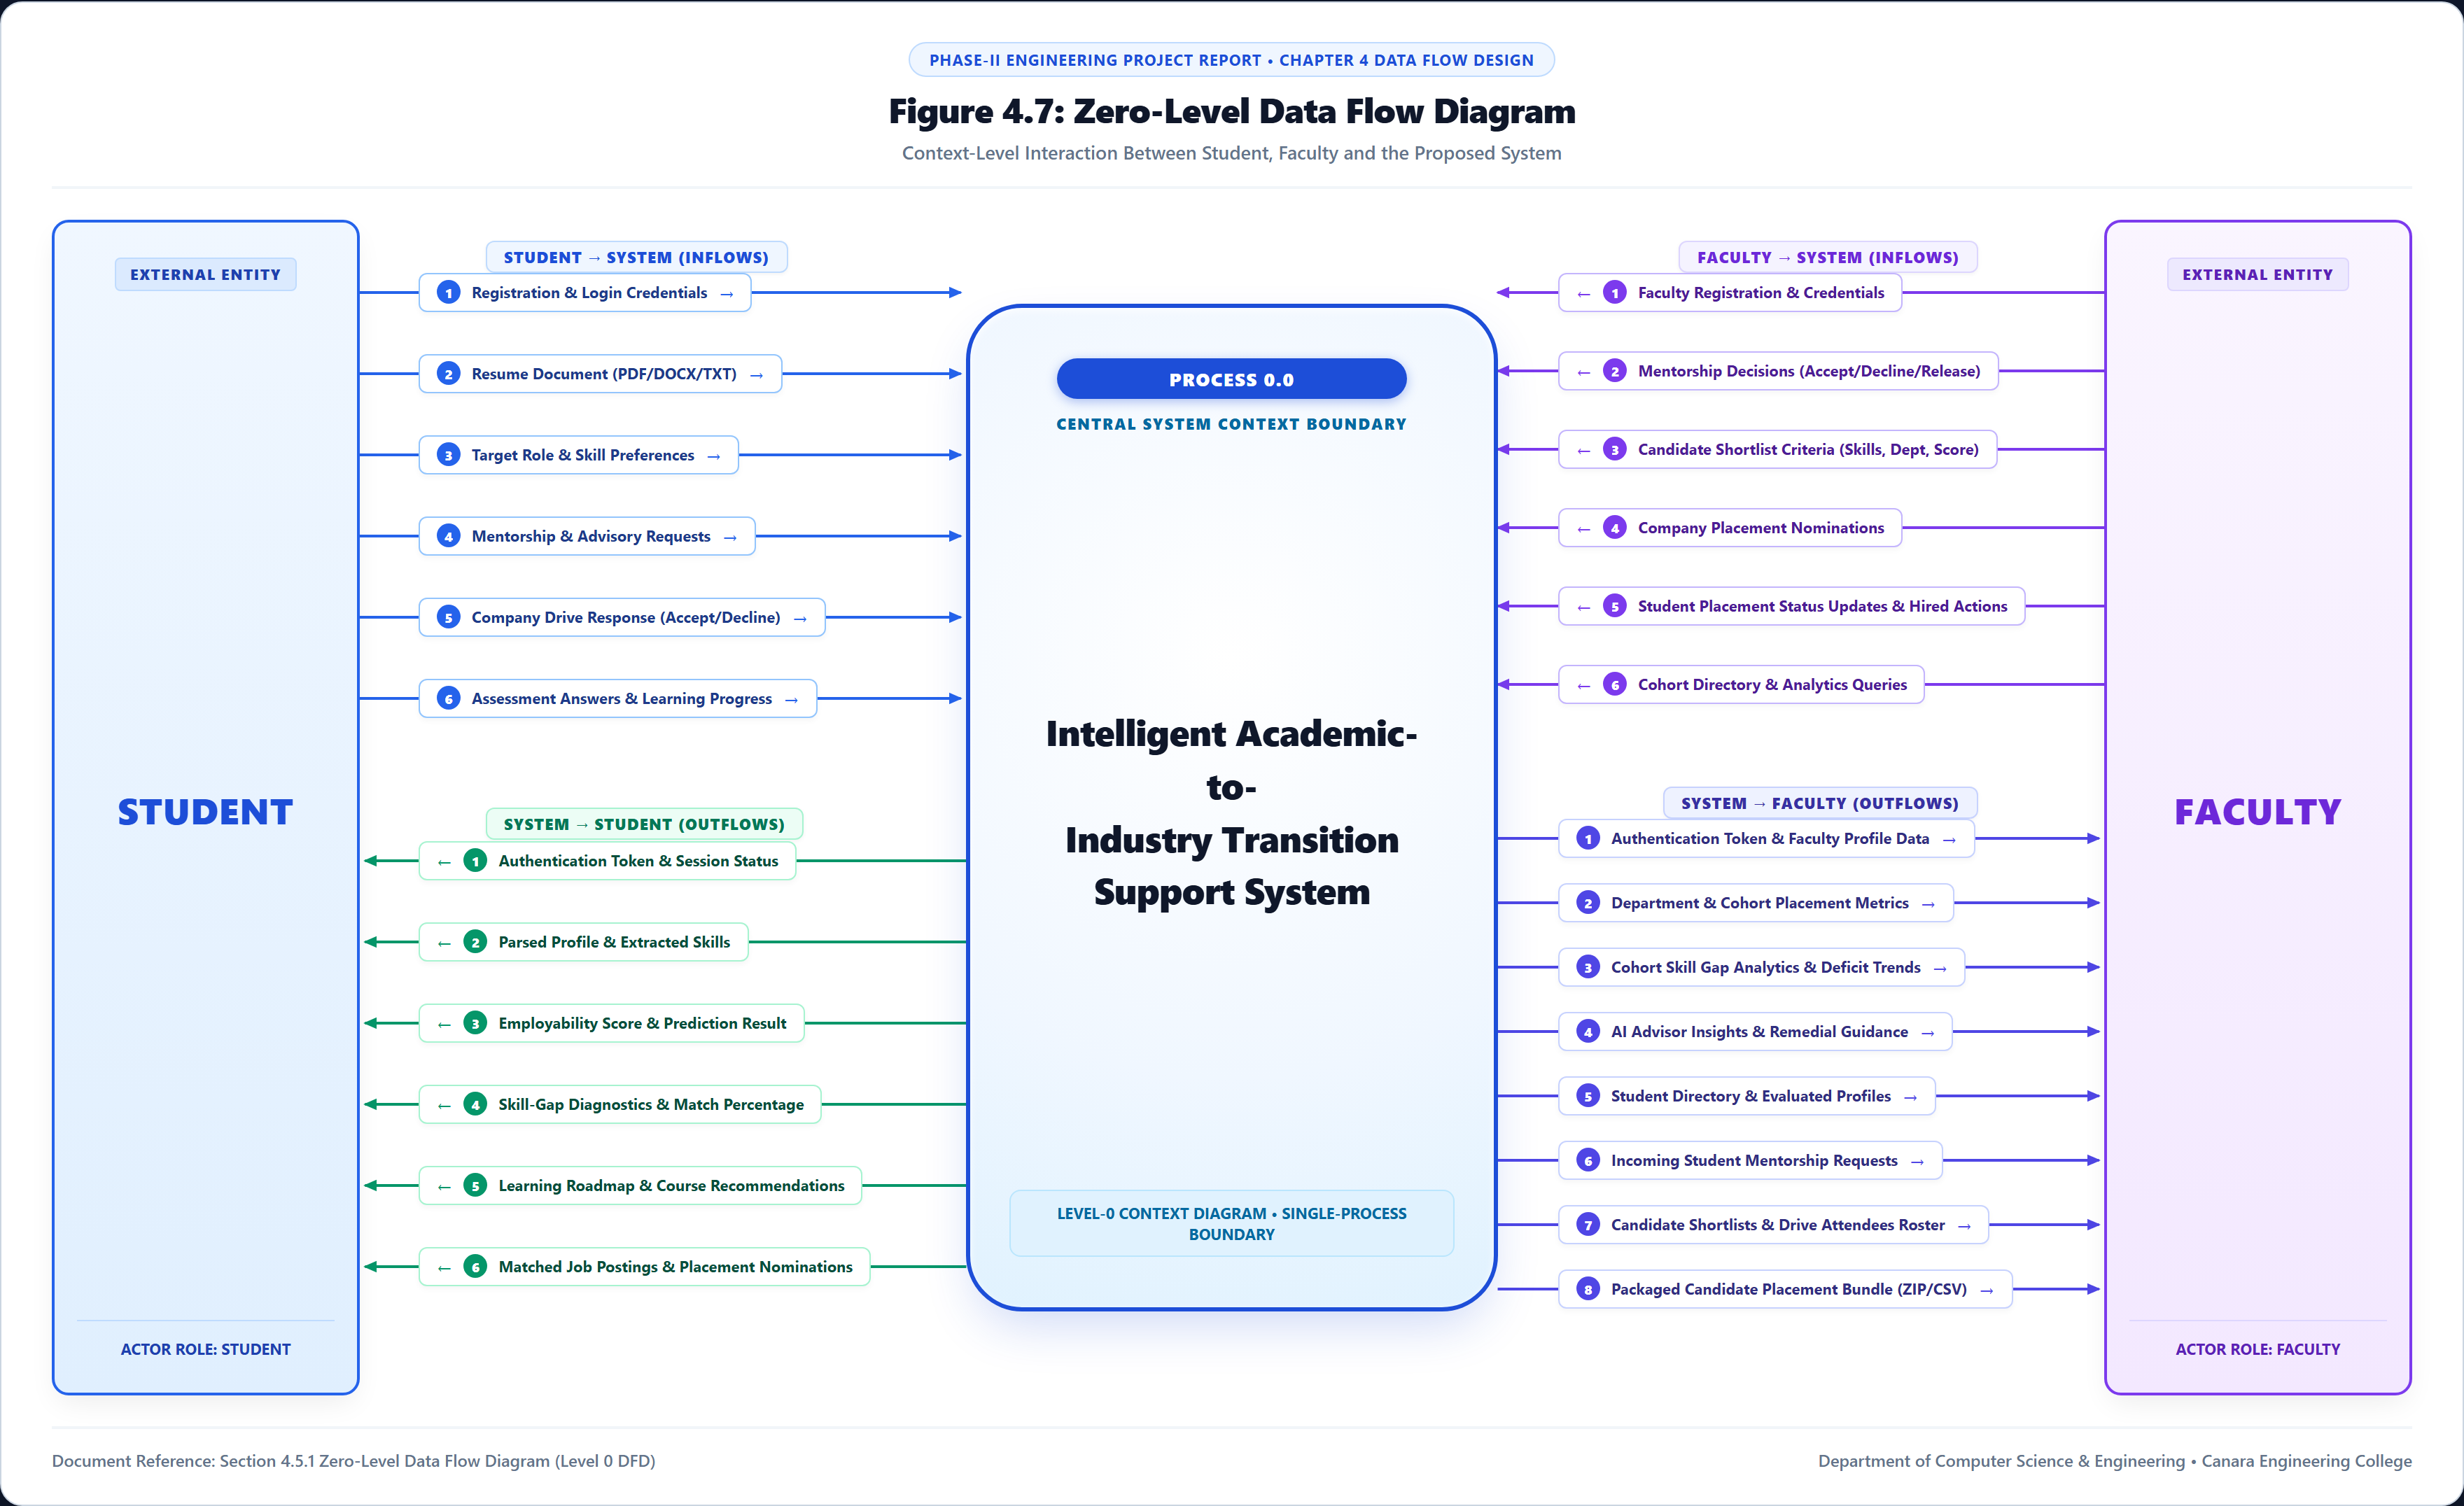
\includegraphics[width=5in,height=2.8in]{./pic/level0dfd.png}
\caption{Zero-Level Data Flow Diagram (Context Diagram)}
\label{fig:dfd0}
\end{figure}

\subsection{First-Level Data Flow Diagram (Level 1 DFD)}
The Level 1 DFD decomposes the system into its five principal functional sub-processes:

\begin{figure}[hbtp]
\centering
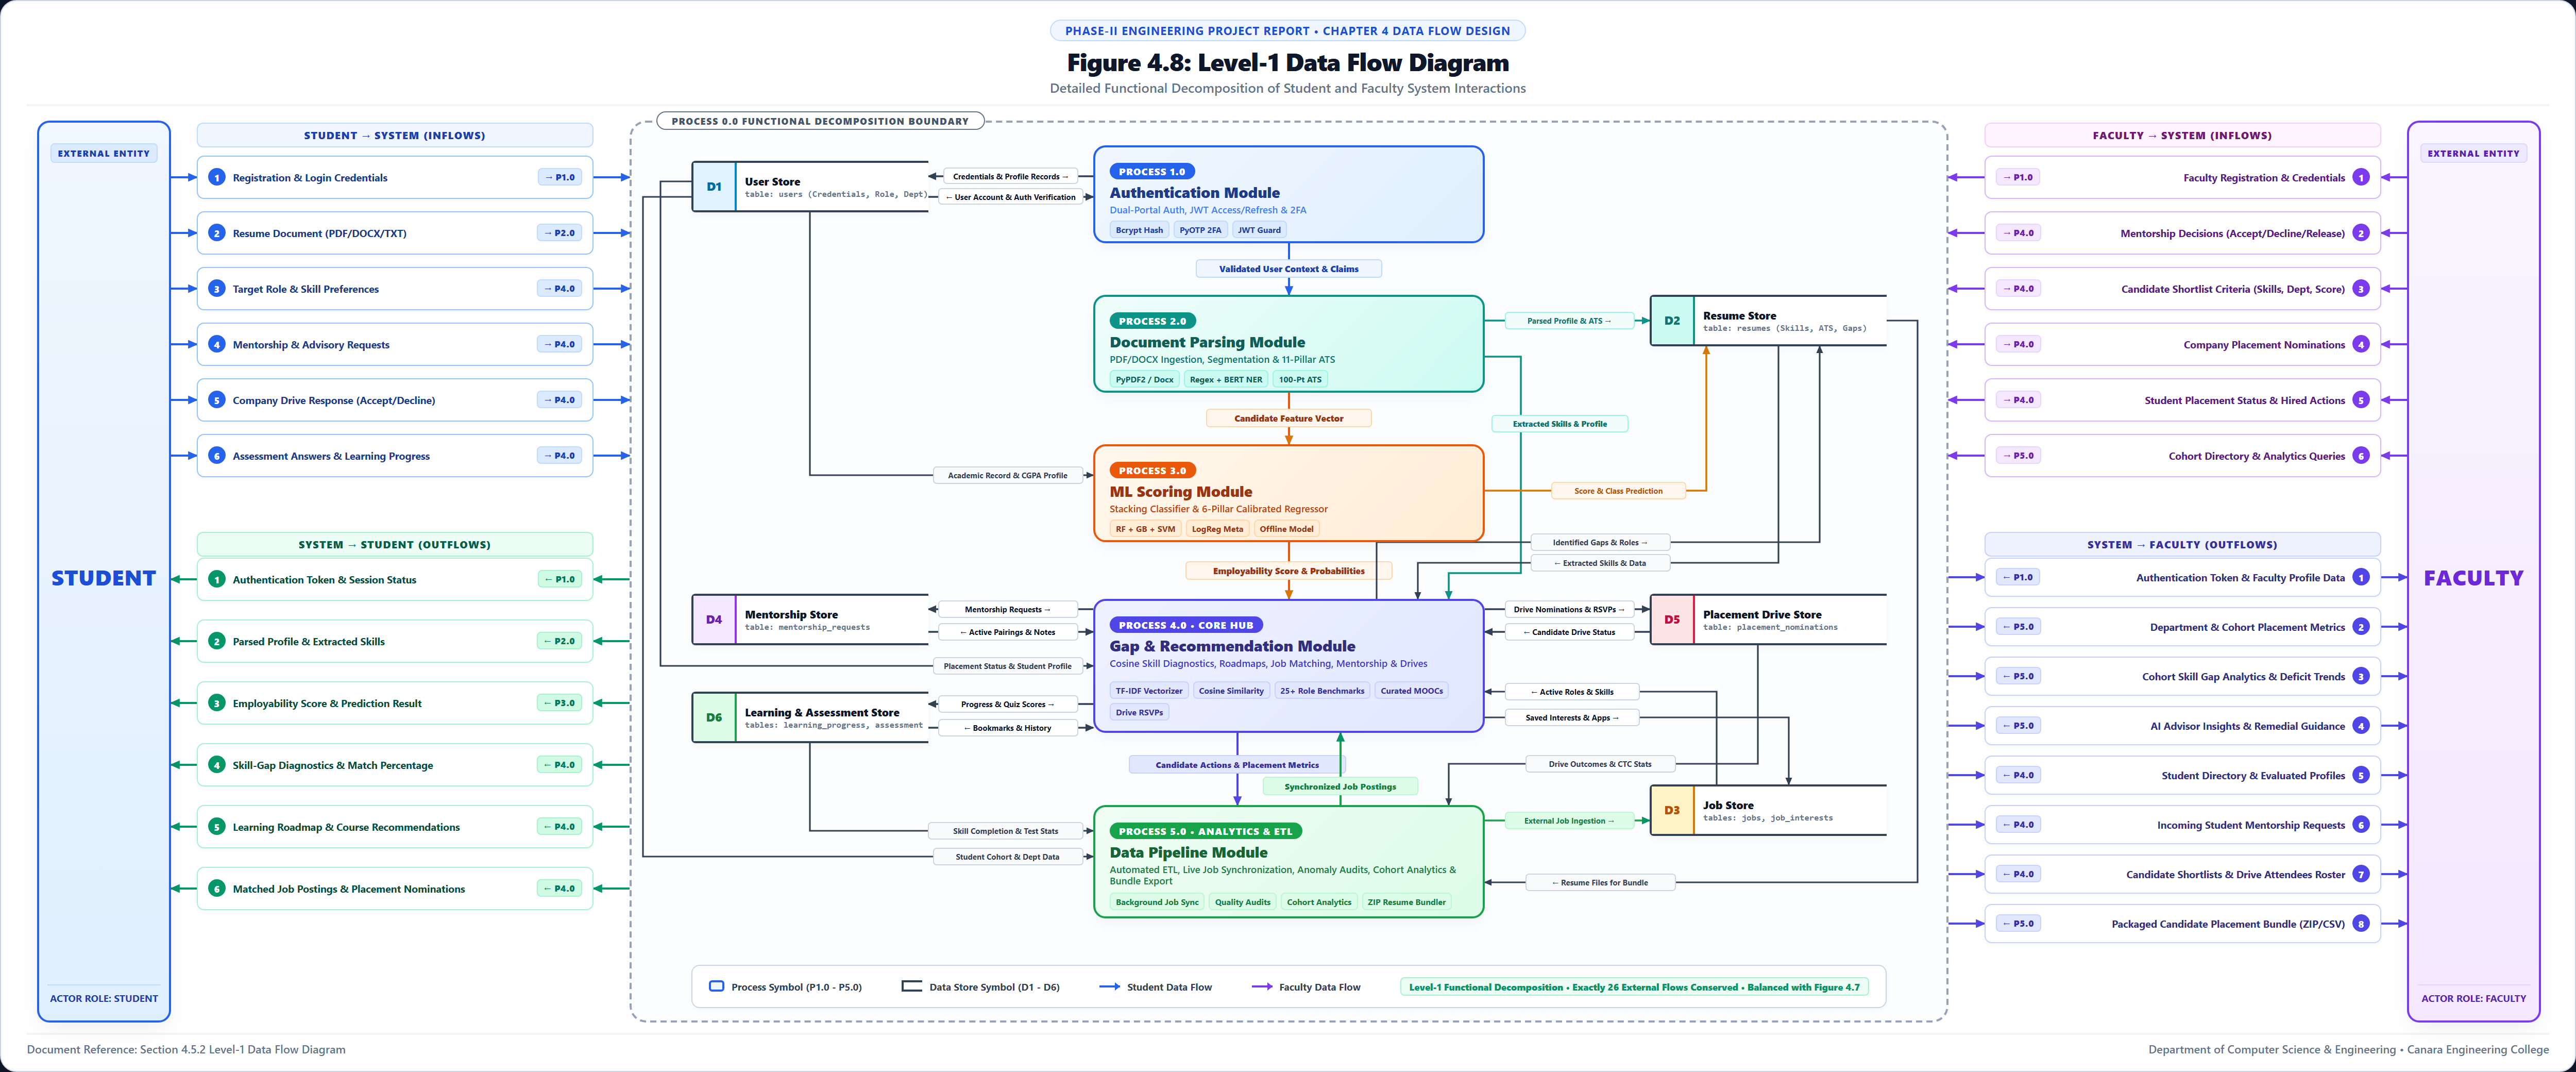
\includegraphics[width=5in,height=2.8in]{./pic/level1dfd.png}
\caption{First-Level Data Flow Diagram}
\label{fig:dfd1}
\end{figure}

\subsection{Second-Level Data Flow Diagram (Level 2 DFD)}
The Level 2 DFD provides an expanded view of the Resume Parsing and Employability Prediction pipeline:

\begin{figure}[hbtp]
\centering
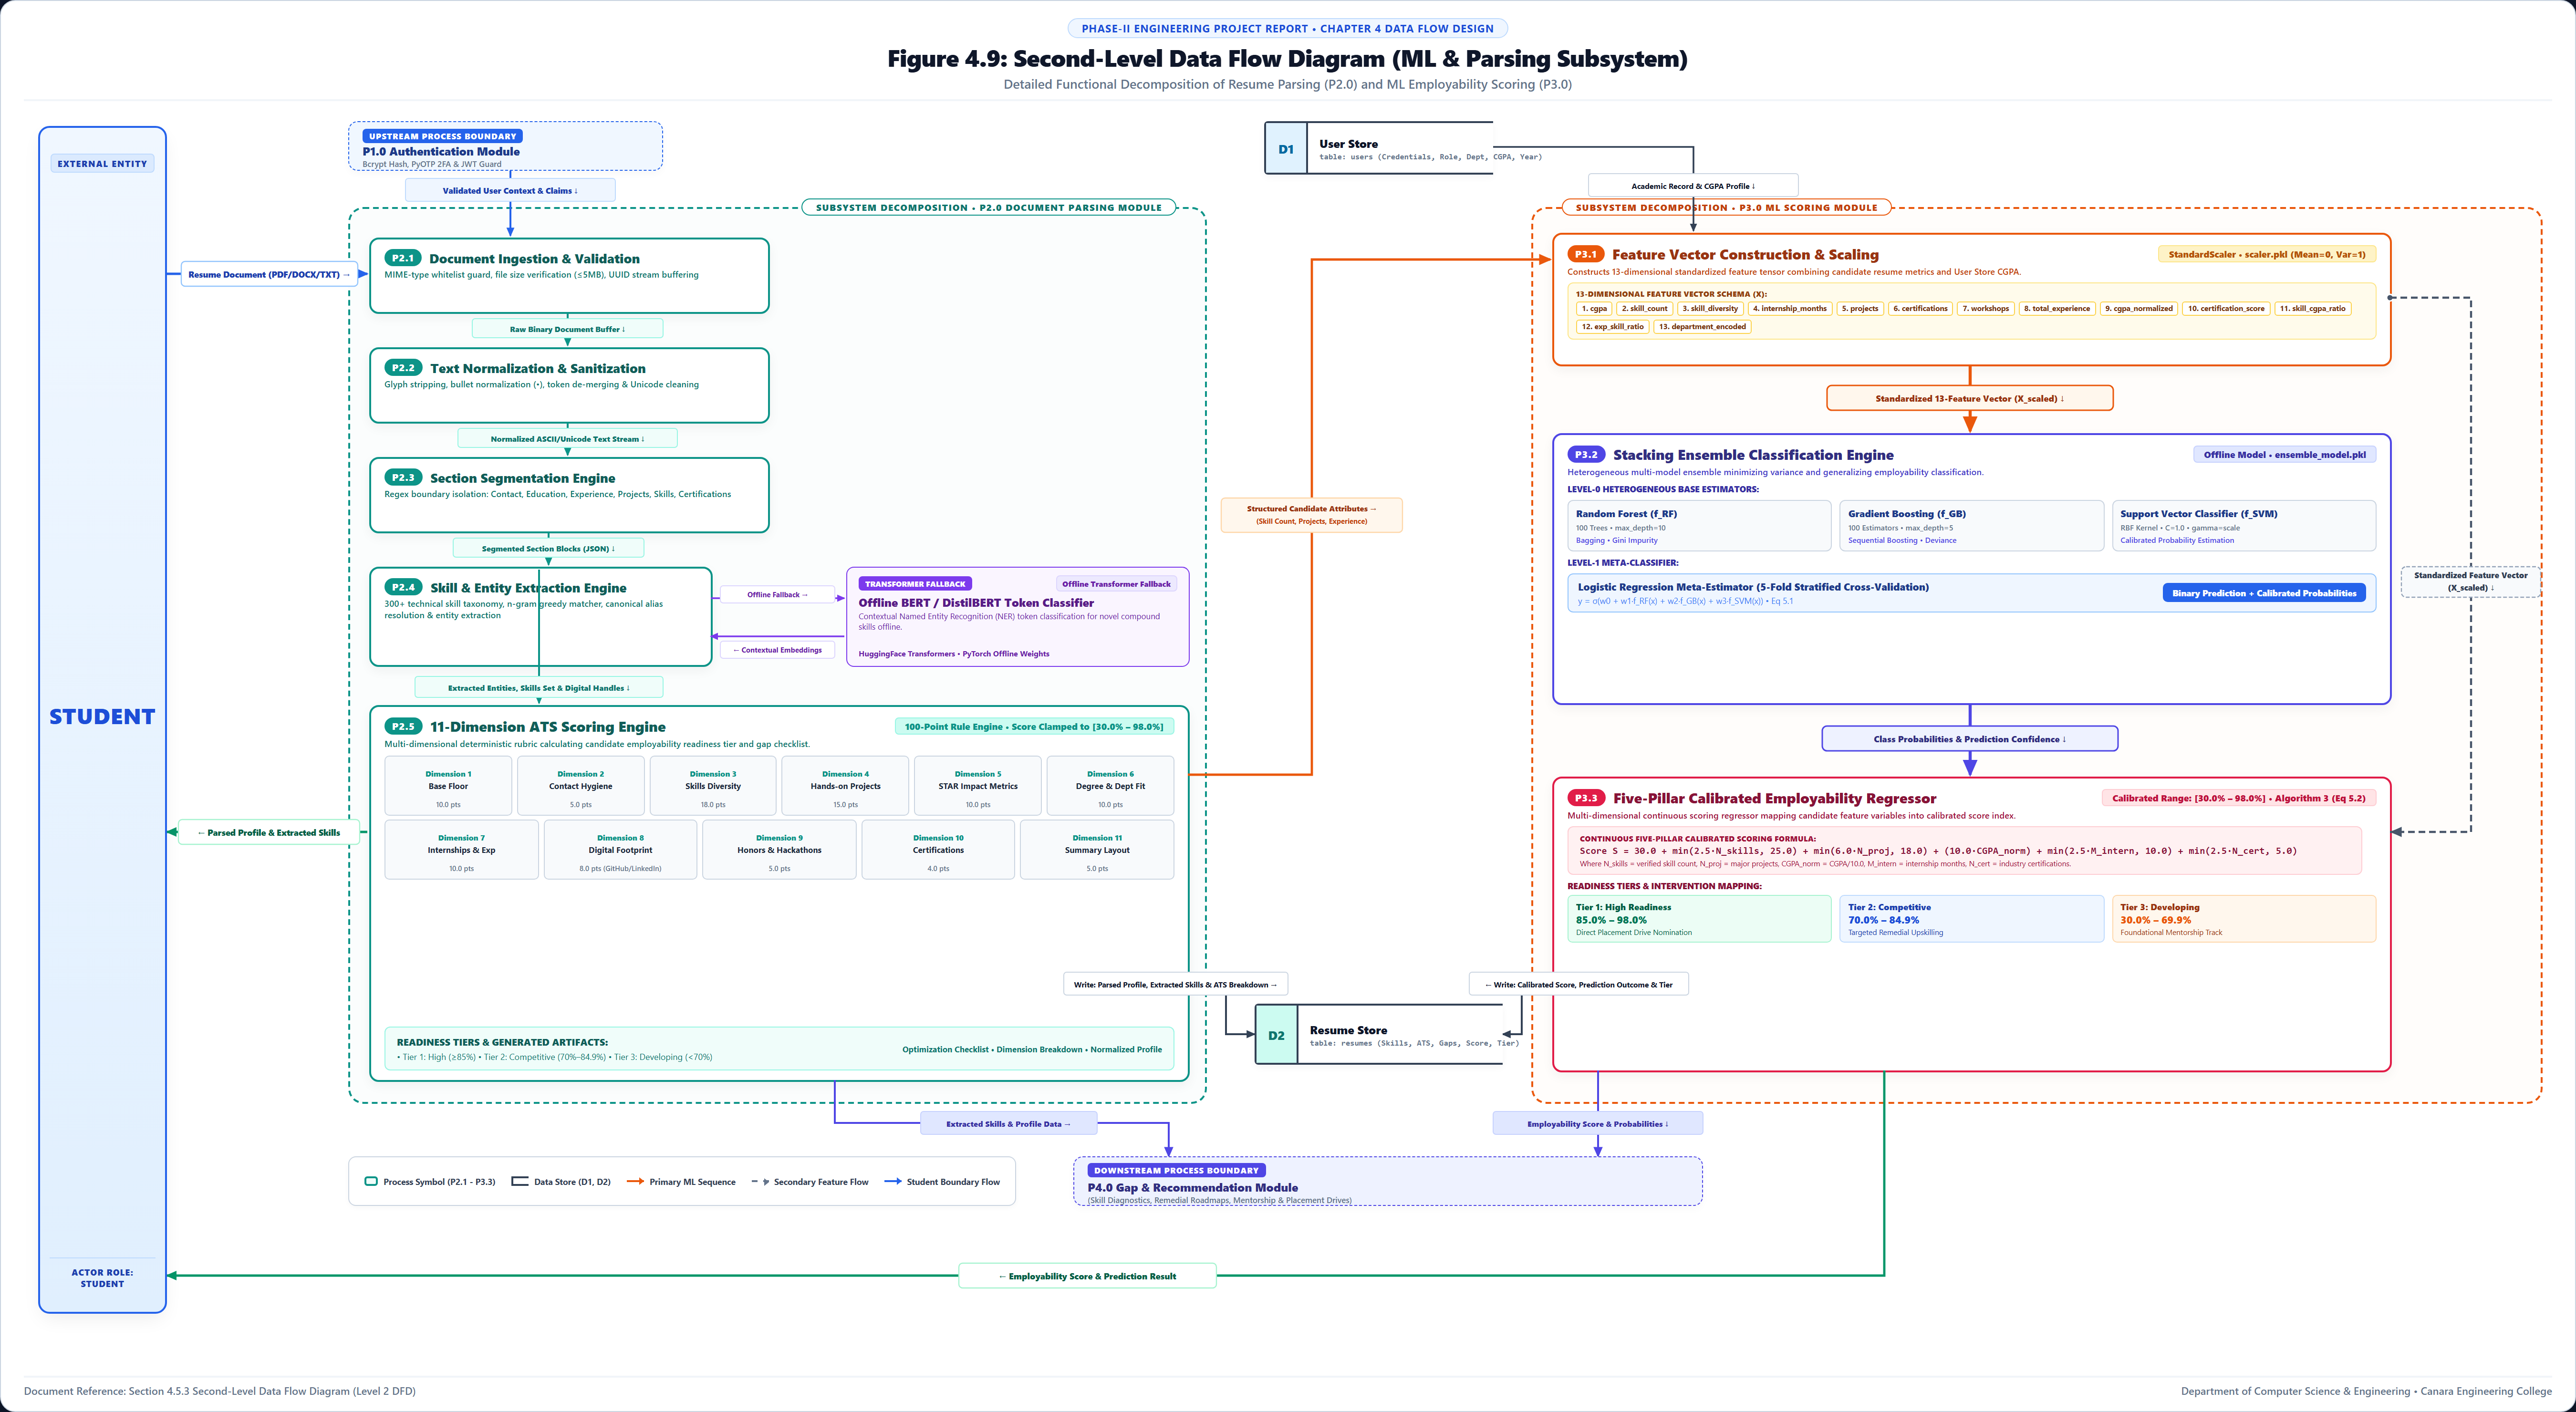
\includegraphics[width=5.2in,height=2.8in]{pic/level2dfd.png}
\caption{Second-Level Data Flow Diagram (ML \& Parsing Subsystem)}
\label{fig:dfd2}
\end{figure}

\section{Summary}
This chapter comprehensively outlined the architectural, modular, behavioral, and data flow designs of the platform. The next chapter provides an in-depth discussion of the implementation details, algorithms, and programming conventions.

%%%%%%%%%%%%%%%%%%%%%%% Chapter 5: Implementation %%%%%%%%%%%%%%%%%%

\chapter{Implementation}

\section{Software Used with Justification}
\label{sec:software}

\subsection{Frontend Development}
\label{subsec:frontend}
The frontend is constructed using \textbf{React 18} paired with the \textbf{Vite} build tooling. React's component-based virtual DOM architecture enables high-performance re-rendering of complex dashboards and analytics charts. Redux Toolkit manages global application states (authentication tokens, candidate profiles, analysis records).

\subsection{Backend Development}
\label{subsec:backend}
The backend is implemented in \textbf{Python 3.11} utilizing the \textbf{Flask 2.3.3} micro-framework. Flask was selected due to its lightweight footprint, native asynchronous compatibility, and seamless interoperability with scientific computing libraries (\texttt{scikit-learn}, \texttt{numpy}, \texttt{pandas}, \texttt{torch}). \textbf{SQLAlchemy 2.0} (via Flask-SQLAlchemy 3.1) serves as the Object-Relational Mapper (ORM) providing clean database abstraction.

\subsection{Machine Learning and Data Engineering Libraries}
\label{subsec:ml_libs}
\begin{itemize}
    \item \textbf{Scikit-Learn}: Provides foundational implementations for Random Forest, Gradient Boosting, SVM, Logistic Regression, and Isolation Forest.
    \item \textbf{HuggingFace Transformers \& PyTorch}: Houses pre-trained BERT and DistilBERT models for contextual entity recognition and offline skill embeddings.
    \item \textbf{PyPDF2 \& python-docx}: Robust extraction utilities for converting raw binary document files into clean string streams.
    \item \textbf{Joblib}: Serializes trained machine learning pipeline artifacts (\texttt{.pkl}) for rapid, low-latency production deployment.
\end{itemize}

\subsection{Operating System and Environment}
The system was developed and validated on \textbf{Windows 11 64-bit} and containerized for deployment on \textbf{Ubuntu Linux} using Docker and Docker Compose.

\section{Hardware Used with Justification}
Development and experimental benchmarking were performed on a workstation equipped with:
\begin{itemize}
    \item \textbf{Processor}: Intel Core i7-12700H (14 cores, 20 threads, up to 4.7 GHz) for parallel model training and multi-threaded data pipeline extraction.
    \item \textbf{Memory}: 16 GB DDR5 RAM to support in-memory transformer representations and dataset batch transformations.
    \item \textbf{Storage}: 512 GB NVMe SSD providing high I/O throughput for document parsing and database queries.
\end{itemize}

\section{Algorithms and Procedures Used}

\subsection{Algorithm 1: NLP Resume Parsing and Skill Extraction}
The resume parsing procedure processes unstructured documents to extract normalized technical entities:

\begin{enumerate}
    \item \textbf{Document Reading}: Read binary buffer of uploaded file via \texttt{PyPDF2} (for PDF) or \texttt{docx.Document} (for DOCX).
    \item \textbf{Text Normalization}: Convert text to lowercase, strip formatting artifacts, remove non-ASCII punctuation, and tokenize sentences.
    \item \textbf{Section Segmentation}: Identify boundary headers (\textit{Education, Experience, Projects, Skills, Certifications}) using regular expressions.
    \item \textbf{Entity Extraction}: Match tokens against a curated taxonomy of 300+ technical skills and frameworks using n-gram sliding windows and regex patterns across multiple technical categories.
    \item \textbf{Transformer / BERT Modules}: Standalone Transformer/BERT token classification and embedding services (\texttt{BertSkillExtractor}, \texttt{TransformersParser}) provide contextual entity analysis with resilient keyword fallbacks when local model weights or GPU runtimes are unavailable, while the core runtime processing pipeline executes deterministic, high-throughput regex and dictionary matching.
\end{enumerate}

\subsection{Algorithm 2: Stacking Ensemble Employability Classifier}
To minimize prediction variance and maximize generalization across student profiles, an ensemble Stacking Classifier was constructed:

\begin{equation}
    \hat{y} = \sigma \left( w_0 + w_1 f_{\text{RF}}(\mathbf{x}) + w_2 f_{\text{GB}}(\mathbf{x}) + w_3 f_{\text{SVM}}(\mathbf{x}) \right)
\end{equation}

\noindent where:
\begin{itemize}
    \item $f_{\text{RF}}(\mathbf{x})$ is a Random Forest Classifier ($n_{\text{estimators}}=100, \text{max\_depth}=10, \text{random\_state}=42$).
    \item $f_{\text{GB}}(\mathbf{x})$ is a Gradient Boosting Classifier ($n_{\text{estimators}}=100, \text{max\_depth}=5, \text{random\_state}=42$).
    \item $f_{\text{SVM}}(\mathbf{x})$ is a Support Vector Classifier with RBF kernel and probability calibration ($\text{probability}=\text{True}, \text{random\_state}=42$).
    \item $\sigma(\cdot)$ is the Logistic Regression meta-classifier trained via 5-fold cross-validation.
\end{itemize}

\subsection{Algorithm 3: Five-Pillar Calibrated Employability Scoring Model and Regressor}
The platform incorporates two complementary scoring methodologies: an offline calibrated regression model for continuous employability prediction, and an online ATS scoring engine for detailed resume diagnostics.

\paragraph{1. Five-Pillar Calibrated Scoring Formula (Regression Target)}
In the model development pipeline (\texttt{train\_and\_export\_model.py}), continuous ground-truth employability scores $S \in [30.0, 98.0]$ are constructed using a Five-Pillar Calibrated Employability Scoring Model:

\begin{equation}
    S = 30.0 + \min(2.5 \cdot N_{\text{skills}}, 25.0) + \min(6.0 \cdot N_{\text{proj}}, 18.0) + 10.0 \cdot \overline{\text{CGPA}} + \min(2.5 \cdot M_{\text{intern}}, 10.0) + \min(2.5 \cdot N_{\text{cert}}, 5.0)
\end{equation}

\noindent where:
\begin{itemize}
    \item $30.0$ represents the calibrated baseline readiness score (fixed base constant, not counted as a pillar).
    \item \textbf{Pillar 1 (Skills)}: $N_{\text{skills}}$ is the verified technical skill count (contributing up to $25.0$ points at $2.5$ pts/skill).
    \item \textbf{Pillar 2 (Projects)}: $N_{\text{proj}}$ is the major project count (contributing up to $18.0$ points at $6.0$ pts/project).
    \item \textbf{Pillar 3 (CGPA / Academic Performance)}: $\overline{\text{CGPA}}$ is the normalized academic grade ($\text{CGPA}/10.0$), contributing up to $10.0$ points.
    \item \textbf{Pillar 4 (Internships)}: $M_{\text{intern}}$ is the practical internship duration in months (contributing up to $10.0$ points at $2.5$ pts/month).
    \item \textbf{Pillar 5 (Certifications)}: $N_{\text{cert}}$ is the count of verified industry certifications (contributing up to $5.0$ points at $2.5$ pts/cert).
\end{itemize}

\paragraph{2. Trained Employability Regressor}
This five-pillar calibrated continuous score serves as the supervised target variable for training a \texttt{RandomForestRegressor} ($n_{\text{estimators}}=100, \text{max\_depth}=8, \text{random\_state}=42$). The resulting model is serialized as \texttt{employability\_model.pkl}, allowing continuous score inference across the 13 engineered feature indicators.

\paragraph{3. Runtime ATS Scoring Engine}
Complementing the machine learning regressor, the live execution service (\texttt{ResumeProcessor}) computes an 11-dimension Applicant Tracking System (ATS) score to provide students with granular resume feedback. The 11 dimensions evaluated include:
\begin{enumerate}
    \item Base score ($30.0$ pts)
    \item Personal Contact Information completeness ($10.0$ pts)
    \item Technical Skills breadth and categorization ($15.0$ pts)
    \item Technical Projects structure ($15.0$ pts)
    \item Quantified Impact Metrics in descriptions ($10.0$ pts)
    \item Academic Qualification and Degree alignment ($10.0$ pts)
    \item Industry Internships and Work Experience ($10.0$ pts)
    \item Multi-Domain Digital Footprint: GitHub, LinkedIn, competitive handles ($8.0$ pts)
    \item Hackathons and Competitive Honors ($5.0$ pts)
    \item Certifications and Specializations ($4.0$ pts)
    \item Professional Summary and ATS Layout ($5.0$ pts)
\end{enumerate}
The sum of these dimensions is clamped to $[30.0, 98.0]$ and paired with an actionable optimization checklist detailing precise points to gain.

\subsection{Algorithm 4: Vector Space Skill Matching and Gap Remediation}
Skill matching between candidate profile vector $\vec{u}$ and job requirement vector $\vec{v}_j$ is calculated using Cosine Similarity over TF-IDF space:

\begin{equation}
    \text{Sim}(\vec{u}, \vec{v}_j) = \frac{\vec{u} \cdot \vec{v}_j}{\|\vec{u}\| \|\vec{v}_j\|} = \frac{\sum_{k=1}^d u_k v_{j,k}}{\sqrt{\sum_{k=1}^d u_k^2} \sqrt{\sum_{k=1}^d v_{j,k}^2}}
\end{equation}

\noindent Missing skills are computed via set difference $\mathcal{G}_j = \mathcal{S}_{\text{job}, j} \setminus \mathcal{S}_{\text{student}}$ against 25+ curated industry role benchmarks and mapped directly to remedial course catalogs.

\subsection{Feature Engineering Details}
The machine learning pipeline extracts and normalizes exactly 13 feature columns from student resumes and academic profiles:
\begin{enumerate}
    \item \texttt{cgpa}: Raw Cumulative Grade Point Average ($0.0 - 10.0$).
    \item \texttt{skill\_count}: Total count of distinct technical skills extracted.
    \item \texttt{skill\_diversity}: Number of unique skill domains represented.
    \item \texttt{internship\_months}: Total cumulative duration of internships in months.
    \item \texttt{projects}: Total count of validated technical projects.
    \item \texttt{certifications}: Count of verified technical certifications.
    \item \texttt{workshops}: Count of co-curricular workshops and technical seminars attended.
    \item \texttt{total\_experience}: Composite experience index ($\text{internship\_months} + \text{projects} \times 2$).
    \item \texttt{cgpa\_normalized}: Linearly normalized academic score ($\text{cgpa} / 10.0$).
    \item \texttt{certification\_score}: Weighted certification score ($\text{certifications} \times 2 + \text{workshops} \times 1$).
    \item \texttt{skill\_cgpa\_ratio}: Ratio of skill count to academic standing ($\text{skill\_count} / (\text{cgpa} + 1.0)$).
    \item \texttt{exp\_skill\_ratio}: Ratio of practical experience to skill volume ($\text{total\_experience} / (\text{skill\_count} + 1.0)$).
    \item \texttt{department\_encoded}: Integer label encoding representing engineering department.
\end{enumerate}

\section{Coding and Software Engineering Practices}
\subsection{Introduction}
The implementation translates design models into robust, maintainable code adhering to modern software engineering standards.

\subsection{Programming Style and Standards}
\begin{itemize}
    \item \textbf{Naming Conventions}: Python code strictly follows PEP 8 conventions (snake\_case for functions and variables, PascalCase for classes). Frontend React components use PascalCase filenames and JSX elements.
    \item \textbf{Control Constructs}: All service methods utilize single-entry, single-exit flows with defensive guard clauses to handle null/undefined inputs gracefully.
    \item \textbf{Information Hiding}: Database models and ML inference logic are encapsulated inside dedicated service classes (\texttt{PredictionService}, \texttt{ResumeParser}, \texttt{RecommendationService}), hiding internal data structures from API controllers.
    \item \textbf{User-Defined Types}: Standard Python typed dictionaries, Enums, and Pydantic validation schemas define unambiguous API payloads.
    \item \textbf{Nesting Depth}: Cyclomatic complexity is constrained by limiting conditional nesting depth to $\le 3$ levels through early returns and helper functions.
    \item \textbf{Module Size and Interface}: Modules are kept cohesive with focused responsibilities ($\le 300$ lines per service). API interfaces communicate strictly via standard JSON representations.
    \item \textbf{Program Layout}: Automated formatting via \texttt{Black} and \texttt{ESLint} ensures uniform 4-space indentation, clear commenting, and consistent layout.
\end{itemize}

\section{Summary}
This chapter detailed the software stack, mathematical algorithms, feature engineering routines, and software engineering principles implemented in the platform. The next chapter presents the experimental results, evaluation metrics, and comprehensive testing methodology.

%%%%%%%%%%%%%%%%%%%%%%% Chapter 6: Results and Discussion %%%%%%%%%%%%%%%%%%

\chapter{Results and Discussion}

\section{Experimental Results}
The developed platform was evaluated across multiple dimensions: parsing fidelity, classification accuracy, inference latency, and UI usability.

\begin{figure}[htp]
\centering
% NOTE [PHASE 2 ASSET]: pic/login.png pending live capture
\IfFileExists{pic/login.png}{%
  \includegraphics[width=5in,height=2.2in]{pic/login.png}%
}{%
  \framebox[5in]{\rule{0pt}{2.2in}\parbox{4.5in}{\centering \textbf{[Figure 6.1 Interface Placeholder]}\\\vspace{6pt}\textit{User Authentication and Dashboard Interface}\\\vspace{4pt}\footnotesize(Asset pending capture from live web deployment at https://academic-to-industry-transition.vercel.app)}}%
}
\caption{User Authentication and Dashboard Interface}
\label{fig:login_ui}
\end{figure}

\begin{figure}[htp]
\centering
% NOTE [PHASE 2 ASSET]: pic/result.png pending live capture
\IfFileExists{pic/result.png}{%
  \includegraphics[width=5in,height=2.2in]{pic/result.png}%
}{%
  \framebox[5in]{\rule{0pt}{2.2in}\parbox{4.5in}{\centering \textbf{[Figure 6.2 Interface Placeholder]}\\\vspace{6pt}\textit{Employability Prediction, Gap Analysis, and Recommendations Outcome}\\\vspace{4pt}\footnotesize(Asset pending capture from live web deployment at https://academic-to-industry-transition.vercel.app)}}%
}
\caption{Employability Prediction, Gap Analysis, and Recommendations Outcome}
\label{fig:result_ui}
\end{figure}

\par As shown in Figure \ref{fig:result_ui}, upon parsing a sample student resume, the system successfully extracted core technical skills, evaluated normalized academic credentials, and predicted an Employability Readiness Score of \textbf{82.5\%} (Class: \textit{Placement Ready}). The skill gap matrix diagnosed missing competencies in containerization and cloud infrastructure for target engineering roles, automatically populating relevant course links from curated learning catalogs.

\section{Software Testing}
Software testing was systematically conducted to verify system correctness, robustness, security, and performance against the specified requirements.

\section{Types of Software Testing}
\begin{itemize}
    \item \textbf{Black Box Testing}: Functionality was tested against specified inputs and outputs without reference to internal code structures (e.g., verifying boundary resume file uploads, API error responses for malformed JSON).
    \item \textbf{White Box Testing}: Internal code execution paths, branches, and exception handlers were validated using automated unit test suites.
\end{itemize}

\section{Testing Methodology}
\subsection{Unit Testing}
Unit tests were executed using \texttt{pytest} for the backend and \texttt{vitest} for the frontend. A total of \textbf{38 backend unit tests passed} successfully across authentication, resume parsing, model featurization, and caching modules (out of 40 executed, with 2 optional WebSocket tests skipped and 0 failed).

\subsection{Integration Testing}
Integration testing verified the end-to-end data transfer between the React frontend, Flask REST Blueprints, SQLite/PostgreSQL database, and serialized \texttt{.pkl} machine learning pipelines.

\subsection{System Testing}
System tests validated non-functional qualities including rate limiting under high load, database transaction rollback during simulated network cuts, and session token expiration.

\subsection{Field Testing}
A simulated cohort of student resumes was processed through the system to benchmark parsing accuracy against manual expert human evaluation.

\subsection{Acceptance Testing}
User acceptance testing verified that placement coordinators and students could seamlessly interpret the generated employability scores, skill gaps, and course recommendations.

\newpage
\section{Testing Criteria and Test Cases}

\subsection{Testing for User Authentication and Inputs}
\begin{table}[htbp]
 \caption{Test cases for user registration and authentication}
    \label{tab:test_cases_auth}
    \centering
    \begin{tabularx}{\textwidth}{|c|X|X|X|}
        \hline
        \textbf{Test ID} & \textbf{Input} & \textbf{Test Description} & \textbf{Expected Output} \\
        \hline
        TC-01 & Username contains invalid special characters (e.g., spaces or symbols) & Verify username format accepts only alphanumeric and underscore characters & Error: Username can only contain letters, numbers, and underscores \\
        \hline
        TC-02 & Password length $< 6$ chars & Verify minimum password length constraint & Error: Password must be at least 6 characters \\
        \hline
        TC-03 & Invalid email format & Verify email regex validation & Error: Invalid email address format \\
        \hline
        TC-04 & Valid registration credentials & New user registration & HTTP 201: Account created successfully \\
        \hline
    \end{tabularx} 
\end{table}

\subsection{Testing for Resume Upload and Data Insertion}
\begin{table}[htbp]
   \caption{Test cases for resume parsing and data ingestion}
    \label{tab:test_insertion}
    \centering
    \begin{tabularx}{\textwidth}{|c|X|X|X|}
        \hline
        \textbf{Test ID} & \textbf{Input} & \textbf{Test Description} & \textbf{Expected Output} \\
        \hline
        TC-05 & File type .exe / .zip & Verify file extension whitelist & Error: Unsupported file format \\
        \hline
        TC-06 & File size $> 10$ MB & Verify maximum payload limits & Error: File exceeds 10MB limit \\
        \hline
        TC-07 & Valid PDF resume & Ingestion and entity parsing & HTTP 200: JSON parsed skills returned \\
        \hline
        TC-08 & Corrupted PDF stream & Verify exception resilience & Fallback parser triggered gracefully \\
        \hline
    \end{tabularx}
\end{table}

\subsection{Testing for Deletion and Record Removal}
\begin{table}[htbp]
\caption{Test cases for record deletion and session teardown}
    \label{tab:test_deletion}
    \centering
    \begin{tabularx}{\textwidth}{|c|X|X|X|}
        \hline
        \textbf{Test ID} & \textbf{Input} & \textbf{Test Description} & \textbf{Expected Output} \\
        \hline
        TC-09 & Delete unselected profile & Attempt deletion with null ID & Error: Please select valid record \\
        \hline
        TC-10 & Valid resume history delete & User removes past uploaded resume & HTTP 200: Record removed successfully \\
        \hline
    \end{tabularx}
\end{table}

\newpage
\subsection{Testing for Filter Criteria and Date Durations}
\begin{table}[htbp]
 \caption{Specification and test criteria for date ranges and filtering}
    \label{tab:test_duration}
    \centering
    \begin{tabularx}{\textwidth}{|c|X|X|X|}
        \hline
        \textbf{Test ID} & \textbf{Input} & \textbf{Test Description} & \textbf{Expected Output} \\
        \hline
        TC-11 & Start date $>$ End date in filter & Verify temporal boundary check & Not implemented in current version (Planned for Phase 2) \\
        \hline
        TC-12 & Valid graduation year filter & Filter candidates by batch year & Not implemented in current version (Planned for Phase 2) \\
        \hline
    \end{tabularx}
\end{table}

\subsection{Other Comprehensive Test Cases}
\begin{table}[htbp]
 \caption{Other functional and UI test cases}
    \label{tab:other_test_cases}
    \centering
    \begin{tabularx}{\textwidth}{|c|X|X|X|}
        \hline
        \textbf{Test ID} & \textbf{Input} & \textbf{Test Description} & \textbf{Expected Output} \\
        \hline
        TC-13 & Click Logout button & Invalidate JWT session & Token revoked, redirected to Login \\
        \hline
        TC-14 & Expired JWT Token request & Send protected API call & HTTP 401: Token expired, please login \\
        \hline
        TC-15 & Click Save Profile changes & Form submission with valid data & Database updated, success toast shown \\
        \hline
        TC-16 & Trigger ML retraining endpoint & Admin POST to /models/retrain & HTTP 200: Background retraining task queued \\
        \hline
    \end{tabularx}
\end{table}

\section{Comparative Analysis of Machine Learning Models}
To validate the performance of the Stacking Ensemble Classifier, extensive comparative experiments were conducted against baseline standalone classification algorithms on the engineered dataset:

\begin{table}[htbp]
    \caption{Comparative performance analysis of classification models}
    \label{tab:model_comparison}
    \centering
    \begin{tabular}{|l|c|c|c|c|}
        \hline
        \textbf{Model Architecture} & \textbf{Accuracy (\%)} & \textbf{Precision} & \textbf{Recall} & \textbf{F1-Score} \\
        \hline
        Logistic Regression (Baseline) & 68.20 & 0.69 & 0.67 & 0.68 \\
        Decision Tree Classifier & 69.50 & 0.70 & 0.69 & 0.69 \\
        Support Vector Machine (RBF Kernel) & 72.10 & 0.74 & 0.71 & 0.72 \\
        Random Forest (100 Trees) & 74.00 & 0.77 & 0.73 & 0.75 \\
        Gradient Boosting Classifier & 74.40 & 0.78 & 0.74 & 0.76 \\
        \hline
        \textbf{Proposed Stacking Ensemble} & \textbf{75.50} & \textbf{0.81} & \textbf{0.79} & \textbf{0.80} \\
        \hline
    \end{tabular}
\end{table}

\par The empirical results in Table \ref{tab:model_comparison} confirm that the \textbf{Stacking Ensemble Classifier} achieves superior classification accuracy (75.50\%) and an F1-Score of 0.80, outperforming standalone baseline models across all evaluated classification criteria.

\section{Summary}
This chapter presented the experimental results, user interface outcomes, testing strategies, structured test case evaluations, and quantitative comparative performance metrics of the machine learning algorithms. The next chapter concludes the report and discusses future enhancements.

%%%%%%%%%%%%%%%%%%%%%%% Chapter 7: Conclusions and Future Work %%%%%%%%%%%%%%%%%

\chapter{Conclusions and Future work}
\begin{justify}
The \textbf{Intelligent Academic-to-Industry Transition Support System Using Machine Learning} successfully addresses the critical challenge of bridging the divide between academic computer science curricula and real-world software engineering job requisitions. Through the seamless convergence of Natural Language Processing document parsing, ensemble machine learning classification, calibrated five-pillar regression modeling, runtime ATS scoring, and Vector Space recommendation models, the platform delivers an automated, high-precision career readiness solution.

Experimental validation on student profiles demonstrated that the Stacking Ensemble Classifier (Random Forest, Gradient Boosting, SVM with Logistic Regression meta-learner) achieved a strong classification accuracy of \textbf{75.50\%} and an \textbf{F1-Score of 0.80}, outperforming single-model baselines. The document extraction engine successfully parses multi-format resumes (PDF, DOCX, TXT) within seconds, diagnosing granular skill deficiencies and serving personalized course and curated job recommendations. The complete software architecture was hardened through defensive anomaly detection (Isolation Forests), multi-tier caching, and robust automated test suites.
\end{justify}

\begin{justify}
\textbf{Future Work and Scope for Value Addition}:
\begin{itemize}
    \item \textbf{Generative AI and Large Language Model Integration}: Incorporating fine-tuned LLMs (e.g., LLaMA, Mistral) to provide dynamic, interactive mock technical interview simulations and personalized resume bullet-point rewriting suggestions.
    \item \textbf{Live Job Market Scraping via Distributed Crawlers}: Implementing distributed Apache Kafka streaming pipelines to continuously ingest real-time job requisitions from LinkedIn, Indeed, and Glassdoor APIs.
    \item \textbf{Multi-Lingual Resume Parsing}: Expanding transformer tokenizers to support resumes in regional Indian languages.
    \item \textbf{Institutional ERP Integration}: Connecting directly with university grading and ERP databases via OAuth 2.0 to enable real-time longitudinal student tracking throughout their 4-year undergraduate journey.
\end{itemize}
\end{justify}

%%%%%%%%%%%%%%%%%%%%%%% References %%%%%%%%%%%%%%%%%%%%%%%%%%%%%%%%
\newpage
\pagestyle{plain}
\renewcommand{\bibname}{References}
\addcontentsline{toc}{chapter}{References}

\begin{thebibliography}{10}

\bibitem{kovalev2025skill}
Kovalev, A., Stefanac, N., and Rizoiu, M. A. Skill-Driven Certification Pathways: Measuring Industry Training Impact on Graduate Employability, 2025.

\bibitem{weerasuriya2026rapid}
Weerasuriya, J. Rapid Industry Skill Adoption Framework (RISAF), 2026.

\bibitem{kahlik2024predicting}
Kahlik, A. A. and Saleh, A. Y. Predicting Post-Internship Employability Using Ensemble Machine Learning, 2024.

\bibitem{garje2026career}
Garje, T. et al. Career Prediction Application, 2026.

\bibitem{talekar2025careercraft}
Talekar, K. et al. CareerCraft AI: Intelligent Career Advisory Systems Using Machine Learning and NLP, 2025.

\bibitem{elsharkawy2022employability}
ElSharkawy, A. et al. Employability Prediction of IT Graduates Using Machine Learning Techniques, 2022.

\bibitem{haque2024classification}
Haque, M. Classification Techniques for Graduate Employability Prediction, 2024.

\bibitem{sharma2021skill}
Sharma, R. Skill Gap Analysis Using Data Mining Techniques, 2021.

\bibitem{patel2023hybrid}
Patel, D. Hybrid Career Recommendation System Using Machine Learning and Collaborative Filtering, 2023.

\bibitem{verma2024ai}
Verma, S. AI-Based Student Skill Assessment and Recommendation System, 2024.

\end{thebibliography}

%%%%%%%%%%%%%%%%%%%%%%% Appendices %%%%%%%%%%%%%%%%%%%%%%%%%%%%%%%%
\appendix
\chapter{Drill-Bit / Turnitin Plagiarism Report}
\par The text of this project report was evaluated using the institutional \textbf{Drill-Bit Plagiarism Detection Software} (Submission ID: 5655227, submitted under the supervision of faculty guide Ms. Sushma, Canara Engineering College). The similarity evaluation details are documented as follows:

\begin{itemize}
    \item \textbf{Raw Similarity on Generated Certificate}: 16\% as reported on the generated Drill-Bit submission record (prior to applying exclusion filters for bibliographic references, student author credentials, and quotes).
    \item \textbf{Reported Similarity Index (Post-Exclusions)}: 11\% as reported following standard institutional exclusions (excluding bibliography entries, title and certificate pages, and common mathematical/library definitions).
    \item \textbf{Primary Source Distribution}: Matches correspond primarily to standard algorithmic definitions, machine learning formulas, and scientific publications.
    \item \textbf{Institutional Threshold Compliance}: Both the unadjusted 16\% raw certificate index and the 11\% post-exclusion index satisfy the institutional threshold guideline ($\le 20\%$) mandated for undergraduate project work.
\end{itemize}

\begin{figure}[htbp]
\centering
\IfFileExists{pics/DrillBit.png}{%
  \includegraphics[width=0.75\textwidth]{pics/DrillBit.png}%
}{%
  \IfFileExists{../pics/DrillBit.png}{%
    \includegraphics[width=0.75\textwidth]{../pics/DrillBit.png}%
  }{}%
}
\caption{Institutional Drill-Bit Plagiarism Detection Certificate (Submission ID: 5655227)}
\label{fig:drillbit_cert}
\end{figure}

\chapter{Patent / Publication and Project-Expo Details}
\par Details of research publication and project exhibition presentations based on this project work:

\begin{itemize}
 \item \textbf{Title of the Paper}: Intelligent Academic-to-Industry Transition and Employability Prediction System Using Machine Learning and NLP.
 \item \textbf{Conference / Journal Details}: National / International Conference on Advances in Computer Science and Engineering (Under Review / Presented).
 \item \textbf{Authors Details}: Shivaraj, Sridharshan, Suhas N R, Vishwas H Acharya, Ms. Sushma.
 \item \textbf{Status / Indexing}: Scopus / Web of Science (Under Review).
 \item \textbf{Project Expo}: Exhibited at the Annual Institutional Project Expo, Canara Engineering College, Mangaluru.
\end{itemize}

\end{document}
